\documentclass[11pt]{article}

% ---------- arXiv-safe standard packages ----------
\usepackage[margin=0.9in]{geometry}
\usepackage{amsmath}
\usepackage{amssymb}
\usepackage{amsthm}
\usepackage{graphicx}
\usepackage{booktabs}
\usepackage{algorithm}
\usepackage{algpseudocode}
\usepackage{float}
\usepackage{placeins}
\usepackage{microtype}
\usepackage[hidelinks]{hyperref}

% ---------- theorem environments ----------
\newtheorem{proposition}{Proposition}
\newtheorem{remark}{Remark}

% ---------- convenience macros ----------
\newcommand{\Class}{\texttt{class}}
\newcommand{\Dfloor}{\Delta_{\text{floor}}}
\newcommand{\Erev}{e^{\text{rev}}}
\newcommand{\Eremax}{e^{\text{rev}}_{\max}}
\newcommand{\Eth}{E_{\text{th}}}
\newcommand{\code}[1]{\texttt{#1}}

\title{COMPASS: Temporally Consistent Topological Passing Decisions for Socially Aware Robot Navigation}
\author{Jungmo Kang \\ \texttt{kangjmo91@gmail.com}}
\date{}

\begin{document}

\maketitle

\begin{abstract}
Service robots in crowded pedestrian environments re-decide, at every control cycle, which side --- left or right --- to pass a person on; when this re-decision is greedy, the passing direction oscillates across cycles in ambiguous configurations, or the robot freezes. This paper proposes COMPASS, a decision-layer planner that treats the \emph{temporal consistency} of passing decisions as a first-class design objective. The passing relationship is represented as a topological \Class\ bound to a person's track ID, stabilizing cross-cycle correspondence, and safety is layered lexicographically on top of a commitment switching rule that unifies the switching margin, dwell, and point of no return into a single \emph{leaky evidence accumulation} equation. We formalize five properties (P1--P5) --- anti-oscillation, switching-rate bound, safety dominance, maneuver completion, and bounded thrashing with safe termination. The anti-oscillation guarantee we claim is \emph{deterministic and pathwise}: at least $N_{\min} = \lceil E_0/((D_{\max}-\Dfloor)\,dt)\rceil$ control cycles separate consecutive discretionary switches (P2), assuming only the range bound $D_k \le D_{\max}$ that the $[0,1]$ cost normalization supplies by construction, together with the declared non-vacuity condition $E_0 > (D_{\max}-\Dfloor)\,dt$ ($N_{\min} \ge 2$), which the default knobs satisfy ($N_{\min} = 3$ cycles in the worst case $D_{\max} = \sum_X w_X$, and $7$ cycles when the advantage is bounded by a single normalized term). P2 bounds the switching rate from above only; a companion response-time bound gives, under a sustained challenger advantage, the finite number of cycles within which a discretionary switch occurs, and it reproduces the mechanism behind the late-reversal and progress-rate freezing findings of the harness. P1 refines this, for i.i.d.\ challenger advantages, to an exponentially small per-cycle switching probability $e^{-\theta^* E_0}$, proved by dominating the accumulator with a Lindley recursion and applying Kingman's bound, where $\theta^*$ is the exact Lundberg root of the increment law and the closed form $\theta^* \approx 2\Dfloor/(\sigma_D^2\, dt)$ serves as tuning guidance only. In measurements from an offline harness that drives the actual decision core (5 scenarios $\times$ 50 seeds), removing the leaky evidence accumulator causes about 98 oscillations per encounter under ambiguous ties, whereas the proposed method commits within $\le 1$; cyclic latency at $K=3$ (8 classes) is p99 $58.6\,\mu s$, max $651.3\,\mu s$ --- only about $1.30\%$ of the 20 Hz budget (50 ms) --- leaving ample decision-core-only real-time margin; and we report a legibility proxy together with a freezing threshold $v_{\text{lat}} \in (0.20, 0.35)\ \text{m/s}$. Physical performance metrics, external baselines, and user studies are not measured; they are specified as a pre-registered protocol in the planned evaluation of \S5.6. The name COMPASS abbreviates \emph{COMmitment-based PASSing for Social navigation}.

\medskip
\noindent\textbf{Keywords:} social navigation, topological path planning, temporal consistency, human-robot interaction, ROS2
\end{abstract}

\section{Introduction}

Autonomous serving, delivery, and guide robots are no longer confined to isolated industrial spaces; they now operate in corridors, lobbies, and sidewalks where people move freely. The central difficulty of such shared spaces is not static-obstacle avoidance but \textbf{interactive passing decisions} with people who continuously change position and intent. In narrow-corridor head-on encounters, situations where the robot overtakes a person or a person overtakes the robot, and crossing-style traversals, the robot must continually judge ``which side to pass on, whether to proceed or yield, whether to stop.''

Widely used local planners (the \texttt{DWA} family, \texttt{MPPI}, \texttt{TEB}) re-optimize a cost function at every control cycle. This greedy re-optimization is natural in static environments, but in ambiguous configurations where the costs of the two passing directions are similar, minor sensor noise or a small movement by the person alone can flip the choice from one cycle to the next. As a result, the robot dithers side to side (oscillation) or, unable to commit to either side, comes to a stop --- an outcome reminiscent of the freezing robot problem \cite{trautman2010}, whose original diagnosis is uncertainty growth rather than commitment failure. Oscillation is not only inefficient --- it also prevents people from reading the robot's intent, undermining both safety and trust.

The central insight of this paper is that the root cause of this problem is not inaccurate perception or prediction but a \textbf{structural defect: the decision policy has no temporal inertia}. Accordingly, rather than investing in a more sophisticated human predictor, we impart explicit temporal consistency to the passing decision itself. The intuition mirrors human walking behavior: once a person decides which way to step aside, they tend to hold that direction, changing it only for a clear reason, and stopping immediately when it becomes dangerous. A related intuition --- that committing to a passing direction aids mutual coordination --- appears in the social-navigation literature as social momentum \cite{mavrogiannis2022momentum}, and this paper embodies the ``hold a once-chosen direction'' behavior as an explicit formal rule at the decision layer.

The contributions of this paper are as follows.

\begin{enumerate}
\item \textbf{ID-indexed representation of topological \Class\ and cross-cycle correspondence.} By binding the identity of a passing direction to a person's track ID rather than to a flickering geometric gap, we consistently identify ``the corridor chosen last cycle'' at every cycle. The spawning, removal, merging, and splitting of \Class{es} caused by people entering, leaving, clustering, and separating are handled via explicit lifecycle rules and TTLs.
\item \textbf{A unified commitment switching rule with a lexicographic safety override.} The switching margin (hysteresis), dwell (persistence), and progress hardening (point of no return) are folded into a single leaky evidence accumulation equation, with safety placed lexicographically above it. This achieves commitment that is ``not rushed, yet not reckless.''
\item \textbf{Formalization of properties and offline empirical validation.} We state anti-oscillation (P1), switching-rate bound (P2), safety dominance (P3), maneuver completion (P4), and bounded thrashing with safe termination (P5) as propositions. The load-bearing anti-oscillation guarantee is P2: a deterministic lower bound of $N_{\min} = \lceil \Eth(\rho)/((D_{\max}-\Dfloor)\,dt)\rceil$ control cycles on the interval between consecutive discretionary switches, holding on every sample path under only the range bound $D_k \le D_{\max}$ that the $[0,1]$ cost normalization of \S4.2 supplies by construction, and informative under the declared design condition $E_0 > (D_{\max}-\Dfloor)\,dt$ ($N_{\min} \ge 2$; Remark~\ref{rem:p2nonvac}). Because P2 is an upper bound on the switching rate and says nothing about switches occurring, we pair it with a response-time bound (Proposition~\ref{prop:p2live}) that gives the finite number of cycles within which a discretionary switch fires under a sustained challenger advantage. P1 refines this, for i.i.d.\ challenger advantages, to an exponentially small per-cycle switching probability and per-unit-time switching rate, proved via Lindley domination and Kingman's bound, with the exponent given by the exact Lundberg root $\theta^*$ of the increment law (the closed form $\theta^* \approx 2\Dfloor/(\sigma_D^2\,dt)$ is retained as tuning guidance only); the exponential form is conditional on that independence hypothesis (\S4.6). P4 is proven, on top of the progress $\rho$ dynamics and a lower bound on the lateral progress rate, via a reachable-upper-bound containment condition on the \textbf{challenger accumulator $\Erev$}. Verification is split into two tiers. The decision layer's behavioral consistency, legibility proxy, and cyclic latency are \emph{measured} using an offline harness that drives the actual decision core, and reported in Chapter 5 (\S5.3, \S5.4); performance metrics requiring physical simulation or a real robot, along with external baselines and user studies, are left as planned evaluations (\S5.6) specified via a pre-registered protocol.
\end{enumerate}

\section{Related Work}

\textbf{Local planners and trajectory optimization.} \texttt{DWA} \cite{fox1997dwa} selects a velocity command from a dynamic window at every cycle; each cycle's selection is made anew, with no memory of previous decisions, so nothing in the scheme itself discourages the chosen side from flipping between cycles (a structural observation of ours, not a claim made in \cite{fox1997dwa}). \texttt{TEB} \cite{rosmann2017teb} maintains and optimizes several topological alternatives in parallel; its ROS implementation adds a selection-cost hysteresis that discourages switching between alternatives, but this is an implementation-level heuristic --- the formulation itself does not define commitment across cycles. \texttt{MPPI} \cite{williams2017mppi} is a sampling-based MPC formulation; it does not treat the discrete structure of social passing decisions as first class. Unlike these, this paper places the temporal consistency of the passing-\Class\ choice itself at the core.

\textbf{Social navigation and proxemics.} The Social Force Model \cite{helbing1995social} describes pedestrian motion as interaction forces, and \texttt{ORCA}/\texttt{RVO} \cite{vandenberg2011rvo} formalizes reciprocal multi-agent collision avoidance; social-navigation work builds on such models of human reactivity and reciprocity when addressing freezing \cite{trautman2010, trautman2015dense}. Proxemics \cite{hall1966hidden} contributes qualitative, culture-dependent interpersonal distance zones, which robotics work has operationalized as cost fields --- notably the asymmetric-Gaussian formulation of Kirby \cite{kirby2010thesis}. While these provide rich human models, they do not treat the oscillation of the robot's decision itself as a measurement target or design goal. This paper adopts such cost fields as input but addresses decision consistency on top of them.

\textbf{HRI navigation --- intent-aware and social momentum.} Intent-aware navigation that estimates human intent and reflects it in planning \cite{trautman2015dense} addresses cooperative driving amid crowds. In particular, social momentum \cite{mavrogiannis2022momentum} scores candidate actions by the angular momentum of the joint robot--human configuration to break mutual deadlocks; it is a per-cycle objective rather than a persistent accumulator, but it articulates the intuition --- committing to a passing side aids coordination --- that this paper formalizes as an explicit scalar evidence accumulator. Metrics for human comfort and social appropriateness are undergoing standardization in social-navigation surveys \cite{mavrogiannis2023survey, gao2022evaluation, francis2023principles}, and this paper takes the axes of decision oscillation and legibility as its quantitative target among these.

\textbf{Pedestrian trajectory prediction.} Learning-based probabilistic predictors --- Social-LSTM \cite{alahi2016sociallstm}, Social-GAN \cite{gupta2018socialgan}, Trajectron++ \cite{salzmann2020trajectron} --- predict a person's future trajectory as a distribution. This paper adopts a Kalman constant-velocity prediction over a short horizon instead (assumptions and limitations in Chapters 3 and 6), but these predictors can be incorporated into this decision layer as a \textbf{replaceable input module}. That is, this contribution is orthogonal to the choice of predictor: as more sophisticated prediction becomes available, only the mean-trajectory and covariance input need be replaced.

\textbf{Topological path planning and passing-side consistency.} H-signature-based enumeration of homotopy classes \cite{bhattacharya2012topological} rigorously represents the topological identity of a path but focuses mainly on static-obstacle topology. The branch that extends this topological view to moving-pedestrian environments is closest to this paper. Dynamic Channel \cite{cao2019dynamicchannel} is a real-time crowd-navigation framework that searches a triangulated spatial graph, combining pedestrian dynamics with topological-corridor selection; it picks one topology per planning cycle but does not formalize the \textbf{temporal consistency} of that choice via an explicit commitment rule or switching-rate guarantee. Winding Through \cite{mavrogiannis2023winding} tracks the homotopy class the robot's path holds relative to each pedestrian and \textbf{penalizes changes to that class over time as a cost} --- being motivated by suppressing passing-side switches, it is the closest prior work to this paper, but it operates as a soft topological-invariance cost internal to the planner and does not define a track-ID-indexed \Class\ lifecycle or a provable switching-rate bound. Topology-driven parallel trajectory optimization \cite{degroot2024topology} runs local MPC optimizers seeded in different homotopy classes in parallel for dynamic obstacles and commits to the best resulting trajectory each cycle, maintaining consistency of the chosen class --- this treats homotopy consistency via parallel search at the trajectory-optimization layer, and does not provide an explicit accumulator-based commitment rule at the discrete decision layer nor a formal switching-rate guarantee for it. Unlike these, this paper places \Class\ correspondence over time (lifecycle) and the commitment rule itself as the object of formalization at the decision layer.

\textbf{Learning-based (IRL) approaches to socially compliant navigation.} The line of work that learns socially compliant costs and prediction models from pedestrian trajectory features via maximum-entropy inverse reinforcement learning \cite{kuderer2012feature, kretzschmar2016irl} models human cooperative avoidance behavior as a trajectory distribution (including a mixture distribution over joint path choices), generating robot trajectories that conform to observed walking conventions. Their contribution is a learned cost/prediction model for trajectory generation; they do not address decision-layer rules or switching-rate bounds that specify how often a discrete passing decision may legitimately flip from cycle to cycle.

\textbf{F-formations and group awareness.} The spatial arrangement people form during conversation/interaction (F-formation) was formalized by Kendon \cite{kendon1990conducting} via the concepts of o-space and p-space; treating such formations as ``groups that must not be split'' is a norm adopted in robot navigation, not part of Kendon's own definition. In robot navigation, detecting and respecting F-formations has been treated as a core element of group-aware navigation \cite{riosmartinez2015survey}. Automatic F-formation detection itself is outside the scope of this paper and is assumed to be provided by an external perception module (details in \S4.8). This paper extends the merge rule of \S4.1 to interaction-based groups so as to avoid splitting F-formations (\S4.8).

\textbf{Legible and predictable motion.} Legible/predictable motion \cite{dragan2013legibility} presents the view that robot motion should reveal intent to an observer. The commitment mechanism of this paper renders motion legible by suppressing decision oscillation, thereby serving as a bridge between the two lines of work. The methodology for human validation of legibility is elaborated via the observer model in \S4.7 and the user-study protocol in Chapter 5.

\textbf{In short}, the problem of temporal consistency on the passing side has been recognized in prior work, with mechanisms of varying explicitness --- a soft topological-invariance penalty \cite{mavrogiannis2023winding}, the selection-cost hysteresis in the ROS implementation of \texttt{TEB} \cite{rosmann2017teb}, per-cycle topological-corridor selection \cite{cao2019dynamicchannel} (one corridor is chosen each cycle, but no cross-cycle commitment is defined), and the social-momentum objective \cite{mavrogiannis2022momentum}. Closest to this paper, \cite{degroot2024topology} \emph{does} formalize inter-cycle topological consistency: a consistency parameter trades off following the previously selected homotopy class against switching to a better one, and at one extreme enforces the previous class as long as it remains valid. The gap this paper fills is therefore narrower than ``no prior work formalizes commitment'', and we state it precisely: combining (i) an explicit lifecycle rule (spawn, removal, merge, split, TTL) that indexes the identity of the passing \Class\ to a person's track ID (defining consistency against person identity rather than against a geometric homotopy class recomputed from the current scene), (ii) a single leaky evidence accumulation switching rule carrying a \emph{deterministic, pathwise} lower bound on the interval between consecutive discretionary switches (P2), together with a conditional exponential refinement of it (P1), and (iii) a lexicographic safety override on top of it (P3) --- combining these three into a single decision layer and presenting them together with formal properties (P1--P5) is, to the authors' knowledge, done here for the first time, and this is the gap this paper fills.

\section{Problem Formulation}

\textbf{Layer separation.} We separate social navigation into three layers. (i) The \textbf{decision layer} --- the layer that determines discrete intents such as which side to pass on, and whether to yield, proceed, overtake, or stop. (ii) The \textbf{trajectory layer} --- the layer that instantiates a given decision as a curvature-continuous ($G^2$) trajectory. (iii) The \textbf{presentation layer} --- the layer that visually reveals the planned trajectory to people (e.g., an AR overlay). The contribution of this paper lies entirely in the \textbf{decision layer}; the trajectory layer adopts an established, validated generator.

\textbf{Notation.} Let $k$ denote the control cycle and $dt$ the cycle interval. Let $\mathcal{C}_k$ denote the set of candidate topological \Class{es} at cycle $k$, and let $J_k(c) \in \mathbb{R}^+ \cup \{\infty\}$ denote the representative trajectory cost of class $c$ ($\infty$ when unavailable). Let $c^*_{k-1}$ denote the previously committed \Class, and let $\mathcal{S}_k = \{c \in \mathcal{C}_k : \mathrm{Safe}_k(c)\}$ denote the safe/available set. Prediction of person $i$ is provided by a Kalman constant-velocity estimator, giving a mean trajectory $\hat p_i(t)$ and covariance $\Sigma_i(t)$, where $\Sigma_i(t)$ grows with the prediction horizon.

\textbf{Assumptions and scope.} (a) Planar (2D) navigation. (b) A short prediction horizon $[0,T]$ (typically 2--4 seconds). (c) Person tracking and data association are provided by an external module. (d) The trajectory generator, given a \Class, corridor, and target speed, is assumed capable of generating a trackable trajectory and of realizing a commanded \textbf{cross-track progress rate} of at least $v_{\text{lat,min}} > 0$ (used in P4). Here $v_{\text{lat,min}}$ is not the vehicle body's lateral (swerve) velocity but the per-unit-time progress rate of the cross-track coordinate toward the planned lateral offset; for non-holonomic drives (differential, Ackermann) it is realized as the product of forward speed and steering (curvature), while for holonomic drives it is realized as a direct lateral-velocity component. Hence $v_{\text{lat,min}} > 0$ presupposes forward clearance and a positive forward speed. (e) Pedestrian passing conventions (e.g., right-side passing) are a locale setting and are not assumed to be a universal constant (Sections 4.2, 5).

\textbf{Objective.} We design a decision policy that guarantees safety at every cycle while ensuring that the passing decision $c^*_k$ does not oscillate unnecessarily, is legible to people, and preserves progress and social comfort.

\section{Method}

\FloatBarrier
\subsection{Enumeration of topological classes and cross-cycle correspondence}

\textbf{Enumeration.} We index the $K$ relevant agents (typically 1--3) within the radius of influence and prediction horizon by track ID. The \Class\ label is defined as a vector of left/right passing signs over each relevant agent.
\begin{equation}
c = (s_{\mathrm{id}_1}, \ldots, s_{\mathrm{id}_K}), \qquad s \in \{L, R\}
\end{equation}
Among the up to $2^K$ combinations, any combination whose corresponding corridor width is narrower than the sum of the robot's width and the safety margin is immediately pruned with $J = \infty$. This corridor-width comparison presupposes a \textbf{circular-footprint approximation} (treating the robot's width as an orientation-independent constant); for elongated rectangular footprints, the occupied area varies with orientation during rotation, making pruning and availability decisions conservative, which we discuss separately in Section 6 (cross-referenced as rectangular-footprint conservatism). The left/right sign of each \Class\ is computed from the winding sign (cross-product integral or H-signature integral) by which the representative path winds around the predicted human positions. Front/rear (temporal-axis) passing is not treated as a separate \Class\ but handled through the asymmetric social cost of Section 4.2. A more rigorous spatiotemporal homotopy extension is discussed as future work in Section 6. The combinatorial explosion of enumeration and the analytical bound on the number of effective \Class{es} after pruning are analyzed in Section 5.4.

\textbf{Cross-cycle correspondence (key).} For ``retain the previous $c^*$'' to be meaningful, $c^*$ must be re-identified every cycle. Because \Class\ identity is bound to track IDs rather than geometry, correspondence reduces to label matching such as ``right of agent \#7, left of agent \#12,'' which rides for free on IDs already provided by the tracking module. Events triggered by human motion are closed by the following rules (Fig.~\ref{fig:lifecycle}).

\begin{itemize}
\item \textbf{Creation} (a relevant agent enters, or a new corridor appears): a new \Class\ appears as a challenger but starts from evidence $e=0$, so there is no immediate jump.
\item \textbf{Extinction} (a relevant agent leaves): the corresponding dimension is removed from all labels. If $c^*$ was distinguished solely by that person, it is absorbed into a coarser \Class; progress $\rho$ is retained if the actual path is unchanged, and reset if it changes.
\item \textbf{Temporary unavailability} (corridor closes, $J=\infty$): identity is retained but passage is momentarily blocked. If $c^*$ is affected, the safety override takes over, and the identity is remembered for a short TTL so that a momentary flicker does not break the commitment.
\item \textbf{Merge} (two people form one cluster): the two dimensions collapse into one, leaving only the sign shared by both sides, with ``between'' becoming $\infty$. The old $c^*$ is mapped to the surviving coarser \Class. Merge decisions use not only spatial proximity but also interaction cues (mutual stillness, mutual orientation, sustained proximity); details are given in \S4.8.
\item \textbf{Split} (a cluster separates): the reverse process --- the old $c^*$ is mapped to the child that is consistent with the robot's current lateral offset and heading.
\end{itemize}

\begin{figure}[t]
\centering
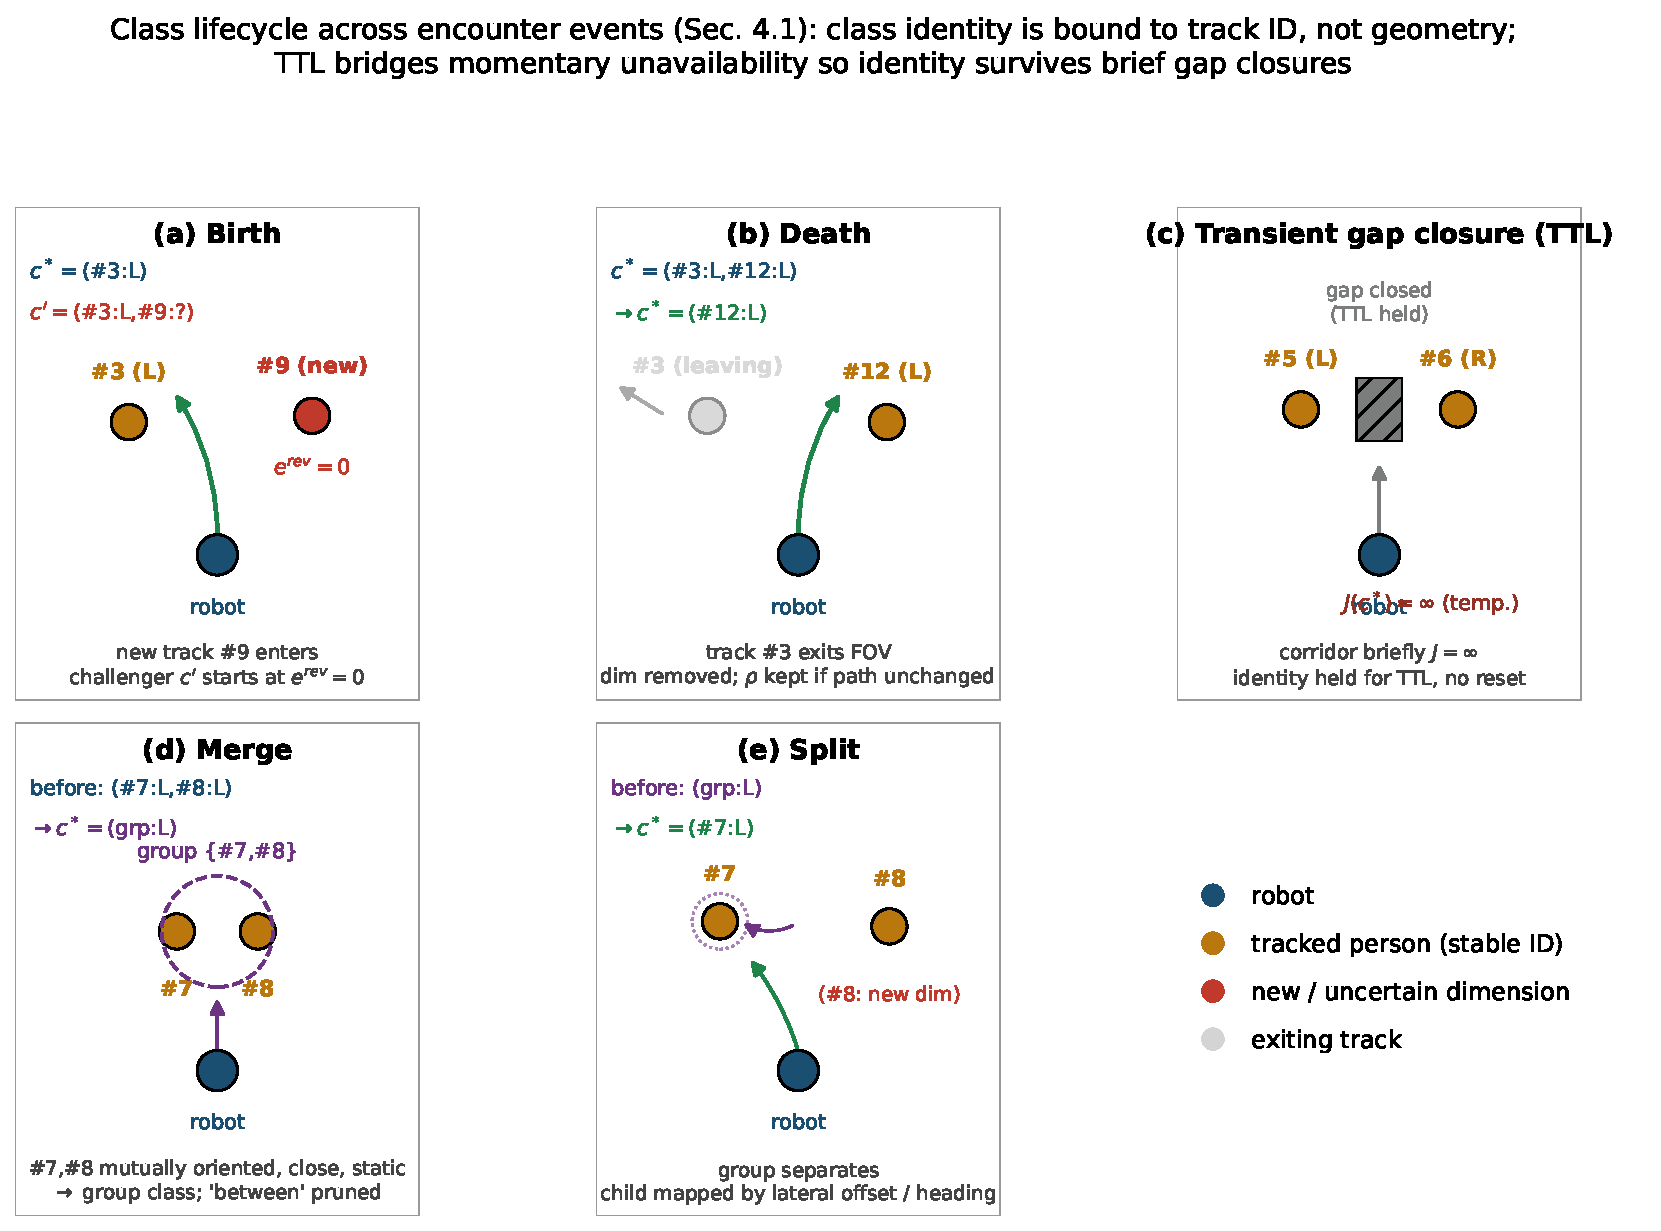
\includegraphics[width=\textwidth]{figures/fig_class_lifecycle.pdf}
\caption{Schematic of the five lifecycle events of a topological class: (a) Creation --- a new track appears as a challenger, starting from $\Erev=0$; (b) Extinction --- when a track leaves, the corresponding dimension is removed ($\rho$ is retained if the path is unchanged); (c) Temporary unavailability --- even when a corridor momentarily becomes $J=\infty$, identity is retained for a TTL to prevent a reset; (d) Merge --- two people judged by interaction cues (mutual orientation, proximity, low speed) merge into a single group class; (e) Split --- a group separates, mapped to the child class consistent with the robot's lateral offset and heading. This emphasizes that class identity is bound to human track IDs rather than geometry.}
\label{fig:lifecycle}
\end{figure}

This structure applies anti-oscillation at two layers: the TTL at the enumeration layer kills the flicker of ``which \Class{es} exist,'' while the accumulator at the decision layer (\S4.3) kills the oscillation of ``which \Class\ is chosen.''

\FloatBarrier
\subsection{Cost function $J(c)$}

The cost of each \Class\ is defined as a weighted sum integrated over the horizon $[0,T]$ along the representative trajectory $\tau_c$.
\begin{equation}
J(c) = w_g J_{\text{goal}} + w_s J_{\text{social}} + w_e J_{\text{effort}} + w_r J_{\text{rule}}, \qquad J(c) = \infty \text{ if unavailable}
\end{equation}

\begin{itemize}
\item \textbf{Progress $J_{\text{goal}}$.} Distance from the local goal $g$ at the end of the horizon: $J_{\text{goal}} = \lVert p_r(T) - g \rVert$. This penalizes detour/stopping \Class{es}.
\item \textbf{Asymmetric social cost $J_{\text{social}}$.} A proxemics cost field is laid over each person and integrated for intrusion (Fig.~\ref{fig:socialcost}).
\begin{align}
J_{\text{social}} &= \sum_i \int_0^T g_i(p_r(t), t)\, dt \\
g_i(p,t) &= \exp\!\left(-\tfrac{1}{2}\, \delta^\top M_i(t)^{-1} \delta\right), \qquad \delta = p - \hat p_i(t) \\
M_i(t) &= R_i(t)\, \mathrm{diag}(\sigma_h^2, \sigma_s^2)\, R_i(t)^\top + \Sigma_i(t)
\end{align}

Here the heading component $\sigma_h$ is set to be front/rear asymmetric ($\sigma_{\text{front}}$ for the front half-plane, $\sigma_{\text{rear}}$ for the rear). This makes the cost of cutting in front of a person differ from that of passing behind them, so that the choice of passing side aligns with social norms. \textbf{$\sigma_{\text{rear}}$ appears in two distinct mechanisms in this paper and must be distinguished. (i) As the base shape of the cost-field asymmetry, $\sigma_{\text{front}} > \sigma_{\text{rear}}$ (the static shape in which the front personal-space region is wider than the rear), and (ii) as a contextual upward adjustment in the overtaking regime (a dynamic adjustment that deliberately raises the rear cost to suppress the surprise of a blind-spot approach) --- these are distinct operating principles: the former induces yielding to the rear in head-on encounters, and the latter suppresses rear approach during overtaking/close passing.} In addition, the predictive covariance $\Sigma_i(t)$ is added to the cost field, so that the personal-space ellipse widens further into the future and the robot gives wider berth accordingly. $\sigma_s$ determines the lateral width. Which of $\sigma_{\text{front}}$ or $\sigma_{\text{rear}}$ applies to a given person is computed from that person's heading and the robot--person relative motion. That is, $\sigma_{\text{front}}$ is applied in the head-on-encounter regime where the robot crosses the person's front half-plane, and $\sigma_{\text{rear}}$ is applied in the overtaking regime where the robot enters the person's rear half-plane; half-plane assignment is determined by projecting $\delta$ into local coordinates referenced to the person's heading. \textbf{Here, the $\sigma_{\text{rear}}$ regime switch (head-on encounter $\leftrightarrow$ overtaking) is not driven by a separate variable but by the same variable as the rear half-plane projection judgment above (the sign of $\delta$'s local projection onto the person's heading) --- that is, the selection of the cost-field asymmetry and the assignment to the overtaking regime are consistently derived from a single judgment.}

\textbf{Parameter grounding and locale configurability.} $\sigma_{\text{front}}$, $\sigma_{\text{rear}}$, $\sigma_s$, and the passing-side preference are not treated as universal constants but as \textbf{locale/culture configuration values}. The basic form of the asymmetric Gaussian proxemics is grounded in Kirby \cite{kirby2010thesis}, and the forward-extended shape draws on Hall's personal-space zones \cite{hall1966hidden} and the social navigation survey \cite{riosmartinez2015survey}. However, we do not adopt the unconditional assumption that ``passing behind is always preferable.'' Since approach from a person's blind spot (rear) can plausibly induce surprise or discomfort --- a design consideration this paper adopts, rather than a finding reported in the surveys cited above --- this cost exposes $\sigma_{\text{rear}}$ as a \textbf{context-dependent knob}, so that (i) rear yielding is preferred in head-on encounters, while (ii) the rear cost is raised during overtaking/close passing to suppress blind-spot entry. The passing-side preference is locale-dependent and configurable (e.g., some pedestrian environments are reported to favor the right, others the left, or a mix). For an experimental study of a single population (Bordeaux, France) showing that avoidance-side conventions in pedestrian crowds can emerge through self-organization, see \cite{moussaid2009experimental}; however, since that study is not a cross-cultural comparison, we do not extrapolate it as direct evidence that ``the passing side varies by culture''; this paper takes the conservative choice of not fixing the passing side as a universal constant but separating it out as a \code{locale.keep\_side} $\in \{\text{right}, \text{left}, \text{none}\}$ setting. The design of the sensitivity analysis for these parameters is described in \S5.5, and their measurement is left to the planned evaluation (\S5.6).

\begin{figure}[t]
\centering
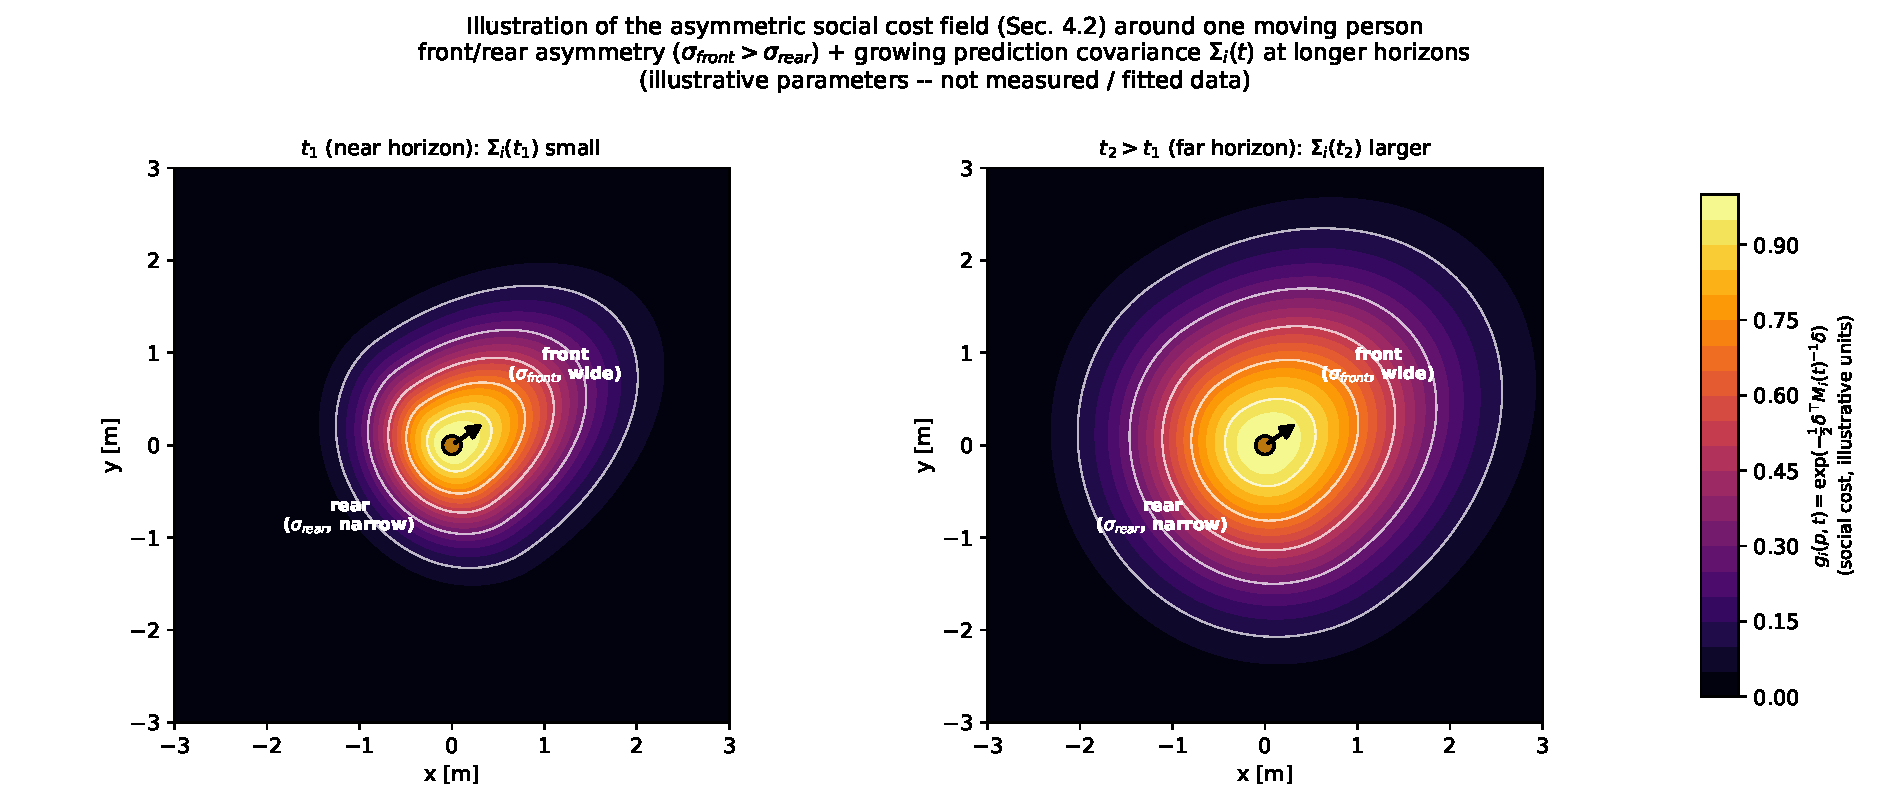
\includegraphics[width=0.85\textwidth]{figures/fig_social_cost_field.pdf}
\caption{Illustrative visualization of the asymmetric social cost field of \S4.2, $g_i(p,t) = \exp(-\tfrac12 \delta^\top M_i(t)^{-1}\delta)$ (a schematic based on the formula, not measured data). Left: near horizon $t_1$ (small predictive covariance $\Sigma_i(t_1)$); right: far horizon $t_2 > t_1$ ($\Sigma_i(t_2)$ grows, expanding the personal-space ellipse). Both panels show the front/rear asymmetry $\sigma_{\text{front}} > \sigma_{\text{rear}}$ (front personal space wider than rear), with half-plane assignment determined by projecting $\delta$ into local coordinates referenced to the person's heading.}
\label{fig:socialcost}
\end{figure}

\item \textbf{Effort/smoothness $J_{\text{effort}}$.} $J_{\text{effort}} = \int_0^T (\alpha \kappa^2 + \beta a^2 + \gamma \dot\kappa^2)\, dt$. The $\dot\kappa$ (curvature rate) term induces $G^2$ continuity, which directly benefits smooth tracking and the curvature display of the presentation layer.
\item \textbf{Rule $J_{\text{rule}}$.} A soft penalty for pedestrian traffic conventions (preference per \code{locale.keep\_side}) and lane keeping. The design of the sensitivity curve for the weight $w_r$ is given in \S5.5.
\end{itemize}

\textbf{Hard availability.} $J = \infty$ if any of the following holds: static collision ($d_{\text{obs}} < r_{\text{safe}}$), insufficient corridor width, violation of kinematic limits, or violation of the hard safety distance $d_{\text{safe}}$ from a predicted person. This is a dual structure in which soft discomfort is handled by $J_{\text{social}}$ while physical/safety constraints are handled by hard availability.

\textbf{Normalization and time-invariance.} If the margin $\Dfloor$ and accumulator threshold $E_0$ are expressed in cost units, they do not port well across scenarios, so each term is normalized to $[0,1]$ against a reference range. Specifically, for a term $X \in \{\text{goal, social, effort, rule}\}$, we normalize $\hat J_X = (J_X - J_X^{\min})/(J_X^{\max} - J_X^{\min})$ and set $J = \sum_X w_X \hat J_X$.

The property guaranteed by the recommended scheme (fixed pre-calibrated constants, below) is \textbf{time-invariance of the normalization map} --- that is, because the normalization constants are fixed regardless of cycle, the meaning of the ``dimensionless advantage'' indicated by $\Dfloor$ is preserved across cycles, and therefore the physical meaning of the margin expressed by the per-cycle $\Dfloor$ remains constant. This is the property that the margin-dependent statements of P1 and P2 actually presuppose.

Here we clarify one distinction. The $J = \sum_X w_X \hat J_X$ immediately after normalization is invariant to the affine rescaling $J_X \mapsto aJ_X + b$ \textbf{with respect to the cost units chosen at calibration time}. However, this affine invariance is limited to the cost units at calibration time, and \textbf{under the fixed-constant scheme, it is broken if the cost units are rescaled after the fact, since the normalization constants do not transform along with the rescaling}. Invariance to cost-unit rescaling is automatically preserved only when the normalization constants co-transform with the units --- that is, only under the per-cycle min--max statistics scheme. The property proved and exploited by the recommended scheme (time-invariance) is therefore distinct from the property the normalization map has with respect to the calibration unit (affine invariance), and the formal properties of this paper rely on the former (time-invariance). This makes the comparison between $\Dfloor$ and $D_k$ consistent across cycles (under the pre-calibrated units).

After normalization, $J$ is dimensionless, so $D_k$, $\Dfloor$, and $E_0$ are all dimensionless, and the product $\Dfloor \cdot E_0$ is likewise dimensionless. Accordingly, in this paper \textbf{$\Dfloor$ is interpreted not as a ``margin in cost units'' but as a fraction of the normalized range $[0,1]$ (a dimensionless switching margin)} (e.g., $\Dfloor = 0.05$ requires a 5\% advantage in the normalized cost range). This interpretation is consistent with all the dimensionless knobs in \S4.3 ($E_0$, $e_{\max}$, $k_\rho$).

\textbf{Choice of $J_X^{\min}\cdot J_X^{\max}$ (time-invariance vs. unit co-variance).} There are two options for the source of the normalization constants, with different implications.

\begin{itemize}
\item \textbf{(Recommended default) Pre-calibrated constants (fixed per scenario).} $J_X^{\min}\cdot J_X^{\max}$ are calibrated once per scenario, independent of the current cycle's candidate set, and then held fixed. In this case the normalization map is invariant across cycles, so the meaning of the ``dimensionless advantage'' indicated by $\Dfloor$ remains constant over time (\textbf{time-invariance} --- the property on which this paper's formal properties rely). Note, however, that as explained above, this scheme loses affine invariance if the cost units are rescaled after the fact, since the normalization constants do not co-transform; it presupposes that the calibration units are fixed and used as such. This paper adopts this as the \textbf{recommended default}.
\item \textbf{(Optional) Per-cycle min--max statistics.} If $J_X^{\min}\cdot J_X^{\max}$ are computed over the current cycle's candidate set $\mathcal{S}_k$, the normalization map changes every cycle along with the candidate set. This scheme automatically preserves \textbf{affine scale invariance} because the normalization constants co-transform with cost-unit rescaling, but at the cost that the actual cost advantage indicated by the same $\Dfloor$ value \textbf{drifts} across cycles. For example, if the candidate set becomes compressed in a given cycle (a narrower min--max range), the same $\Dfloor$ will come to require a larger real cost advantage, so the switching margin that was intended to be fixed effectively becomes time-varying as a function of candidate-set fluctuation. This drift weakens the ``fixed $\Dfloor$ (time-invariant map)'' assumption presupposed by the margin-related statements of P1 and P2, so if per-cycle statistics are used, their effect must be separately measured and bounded in \S5.5.
\end{itemize}

In short, the two options trade off ``time-invariance of the normalization map (recommended; but presupposes fixed calibration units)'' against ``affine invariance from cost-unit co-variance (optional; but accompanied by drift in margin meaning),'' and this paper's formal properties (P1, P2) are stated presupposing pre-calibrated constants (a time-invariant map). This normalization is also the premise for the cross-scenario portability of the switching margin $\Dfloor$ in \S4.3.

\FloatBarrier
\subsection{Commitment switching rule}

Let the challenger be $c'_k = \operatorname*{argmin}_{c \in \mathcal{S}_k,\, c \ne c^*} J_k(c)$, and the challenger advantage $D_k = J_k(c^*_{k-1}) - J_k(c'_k)$. We integrate the margin, dwell, and progress hardening into a single leaky-evidence-accumulation equation.
\begin{align}
e_k &= \mathrm{clip}\big(\lambda\, e_{k-1} + (D_k - \Dfloor)\, dt,\ 0,\ e_{\max}\big) \\
\text{Switching condition:}\quad & e_k \ge \Eth(\rho_k) \\
\Eth(\rho) &= E_0 \cdot (1 + k_\rho \rho^p), \qquad p \ge 1 \\
\rho_k &= \mathrm{clip}\!\left(\frac{|\text{realized cross-track progress}|}{|\text{planned lateral offset of } c^*|},\ 0,\ 1\right)
\end{align}

Here $\Dfloor$ is the instantaneous margin (a dimensionless fraction of the normalized range per \S4.2; advantage beyond this is dissipated by leak $\lambda \in (0,1]$), $\Eth$ is the persistence requirement (dwell), and $k_\rho \rho^p$ is progress hardening (point of no return). An equivalence relation gives intuition. If $\lambda = 1$ and the advantage is a constant $\bar D > \Dfloor$, then $e$ grows as $(\bar D - \Dfloor)t$, switching at $t = \Eth/(\bar D - \Dfloor)$; hence the larger the advantage, the faster the switch (proportional urgency), and as $\Eth \to 0^+$ this reduces to a pure margin, while a large $\Eth$ means a long dwell. When the challenge target changes ($c'$ changes), we reset $e \leftarrow 0$, and at the moment of switching/committing, we reset $e \leftarrow 0, \rho \leftarrow 0$.

Here, $\Dfloor$ is a dimensionless switching margin under the normalization premise of \S4.2, and its absolute meaning is held constant across cycles only when the normalization constants are fixed as pre-calibrated constants (time-invariance of the normalization map) (see the drift analysis in \S4.2). If per-cycle min--max statistics are used, the effective margin of the same $\Dfloor$ drifts with the candidate set, so care is needed in interpreting margin-dependent statements such as the safety dwell and the switching-rate lower bound.

The linear case ($p=1$) hardens uniformly, while the superlinear case ($p>1$) is a ``point of no return''-emphasizing form that allows slack through the middle of the maneuver but locks sharply near the end.

\textbf{Challenger tie-breaking.} If $c'_k = \operatorname*{argmin}$ is not unique (two challengers' normalized costs are tied within numerical tolerance $\varepsilon$), the argmin can waver from cycle to cycle, and the $c' \ne \text{prev}_{c'}$ reset becomes a new source of oscillation that disturbs the accumulator. To prevent this, when tied, we fix a single challenger by the following \textbf{deterministic priority order}.

\begin{enumerate}
\item \textbf{Prefer the previous challenger.} If the previous cycle's $c'$ ($\text{prev}_{c'}$) is in the current tied set, select it (temporal consistency of challenger identity). Because this priority rule applies only within a set of costs tied within the exit threshold $\varepsilon_{\text{out}}$, choosing $\text{prev}_{c'}$ costs no more than $\varepsilon_{\text{out}}$ (the hysteresis exit threshold) relative to the optimal challenger --- i.e., it does not sacrifice more than $\varepsilon_{\text{out}}$ of optimality (consistent with the $\varepsilon_{\text{in}} < \varepsilon_{\text{out}}$ entry/exit hysteresis in the paragraph below).
\item \textbf{Topological distance from $c^*$.} Otherwise, select the challenger with the \textbf{smaller} label Hamming distance (number of differing signs) from the current commitment $c^*$ (preferring the adjacent \Class\ with lower switching cost).
\item \textbf{Deterministic lexicographic order.} If still tied, select the smallest by lexicographic order of \Class\ labels (ascending ID, with $L < R$ at each position).
\end{enumerate}

Because this rule is deterministic, $c'$ does not waver across cycles within a tied configuration, eliminating the artificial oscillation caused by accumulator resets. Meanwhile, $e \leftarrow 0$ fires only when $c'$ genuinely changes (an advantage reversal, not a tie).

\textbf{Hysteresis at the tie boundary itself.} Because boundary chattering can also occur at the tie threshold $\varepsilon$ itself (if the cost difference wobbles near $\varepsilon$, ``tied $\leftrightarrow$ untied'' can flicker across cycles), we place entry/exit hysteresis on the $\varepsilon$ boundary. That is, we separate the threshold $\varepsilon_{\text{in}}$ at which two challengers \textbf{enter} a tied set from the untied state and the threshold $\varepsilon_{\text{out}}$ at which they \textbf{exit} the tied set, with $\varepsilon_{\text{in}} < \varepsilon_{\text{out}}$, so that once a pair of challengers is bound as tied, they are only released as untied when their cost difference exceeds $\varepsilon_{\text{out}}$. This blocks the secondary oscillation in which the tiebreak's own activation/deactivation wobbles at the boundary.

\textbf{Conservatism trade-off of the safety dwell.} The safety dwell and progress hardening of \S4.4 reduce oscillation by delaying switching, but at the cost of equally delaying the response when a genuinely better alternative appears. That is, increasing $\Dfloor \cdot E_0 \cdot k_\rho$ strengthens anti-oscillation but increases the delay of legitimate replanning (conservatism), and this trade-off's operating point is tuned via the sensitivity analysis of \S5.5.

\FloatBarrier
\subsection{Safety override}

Safety/availability is judged by $\mathrm{Safe}_k(c) = [\text{clearance} \ge d_{\text{safe}}] \wedge [\text{TTC} \ge \text{TTC}_{\min}] \wedge [\text{kinematically feasible}]$. If the committed $c^*$ leaves the safe set, all accumulation and hardening from \S4.3 are entirely disregarded (margin is zero in an emergency), and the system drops down the following ladder.

\begin{enumerate}
\item Switch to a safe alternative \Class\ (if one exists).
\item Otherwise, decelerate to buy time.
\item If still hazardous, stop and yield (stopping is always a safe fallback and a legible action).
\end{enumerate}

\textbf{Hysteresis on the safety branch itself.} If the safety ladder chatters at stage 1 (switching) --- i.e., high-frequency repeated safety switches --- this itself becomes a new source of oscillation. To prevent this, we also impose minimal hysteresis on the safety branch. (i) \textbf{Safety dwell.} During a brief protection window $T_{\text{safe\_dwell}}$ immediately following a safety switch, further safety switches are blocked; if the violation persists, the system falls straight through to stage 2 (deceleration). That is, ``if a safety switch was just attempted and safety is immediately violated again,'' the system does not chatter at stage 1 again but transitions to \textbf{deceleration priority}. (ii) \textbf{Deceleration-priority condition.} If the number of safety switches within the preceding window exceeds a threshold (a partial threshold of $N_{\text{thrash}}$ below), stage 1 is skipped and the system starts directly from stage 2. As a result, the safety branch descends monotonically as ``switch $\to$ decelerate $\to$ stop,'' and chattering at stage 1 is structurally blocked.

\textbf{Thrash guard.} If safety-triggered switches occur $N_{\text{thrash}}$ times within a window $W$ (a genuinely ambiguous/deadlocked situation), flailing is stopped and the system drops into stop-and-wait (HOLD). This blocks the reciprocal-dance pathology caused by mutual ambiguity. On re-entry, the system commits to the new best \Class\ and resets $e$, $\rho$, and the dwell timer.

\FloatBarrier
\subsection{Integrated algorithm and trajectory interface}

\begin{algorithm}[H]
\caption{COMPASS decision-layer control cycle (Fig.~\ref{fig:decisionflow})}
\label{alg:compass}
\begin{algorithmic}[1]
\State \textbf{State:} $c^*, e, \rho, n_{\text{thrash}}$ (window $W$), $\text{prev}_{c'}, t_{\text{safe\_dwell}}, \text{mode}$
\For{each cycle $k$}
  \State $\{\hat p_i(t), \Sigma_i(t)\} \leftarrow$ Kalman constant-velocity; \ $\mathcal{C} \leftarrow$ class enumeration (pruned)
  \For{$c \in \mathcal{C}$}
    \State $J(c) \leftarrow w_g \hat J_{\text{goal}} + w_s \hat J_{\text{social}} + w_e \hat J_{\text{effort}} + w_r \hat J_{\text{rule}}$ \quad (each $\hat J_X \in [0,1]$ normalized as in \S4.2, the horizon integrals living inside $J_X$; $\infty$ if unavailable)
  \EndFor
  \State $\mathcal{S} \leftarrow \{c : \text{clearance} \ge d_{\text{safe}} \wedge \text{TTC} \ge \text{TTC}_{\min} \wedge \text{feasible}\}$
  \Comment{\textbf{[Safety]}}
  \If{$c^* \notin \mathcal{S}$}
    \State $n_{\text{thrash}} \mathrel{+}= 1$
    \If{(safety dwell protection active) \textbf{or} (safety switches within window $\ge$ partial threshold)}
      \State $v_{\text{cmd}} \leftarrow \max(0, v_{\text{cmd}} - a_{\text{brake}} dt)$; \textbf{if} $\text{TTC} < \text{TTC}_{\text{stop}}$ \textbf{then} mode $\leftarrow$ STOP \Comment{deceleration priority}
    \ElsIf{$\mathcal{S} \ne \emptyset$}
      \State $c^* \leftarrow \operatorname*{argmin}_{c \in \mathcal{S}} J(c)$; $e \leftarrow 0$; $\rho \leftarrow 0$; $t_{\text{safe\_dwell}} \leftarrow T_{\text{safe\_dwell}}$ \Comment{safety switch + dwell}
    \Else
      \State $v_{\text{cmd}} \leftarrow \max(0, v_{\text{cmd}} - a_{\text{brake}} dt)$; \textbf{if} $\text{TTC} < \text{TTC}_{\text{stop}}$ \textbf{then} mode $\leftarrow$ STOP
    \EndIf
    \If{$n_{\text{thrash}} \ge N_{\text{thrash}}$} mode $\leftarrow$ HOLD \EndIf
  \Else
    \Comment{\textbf{[Discretionary]}}
    \State $c' \leftarrow \textsc{TieBreak}(\operatorname*{argmin}_{c \in \mathcal{S}, c \ne c^*} J(c),\ \text{prev}_{c'},\ c^*)$ \Comment{tie-break ($\varepsilon_{\text{in}}/\varepsilon_{\text{out}}$ hysteresis)}
    \State $D \leftarrow J(c^*) - J(c')$
    \If{$c' \ne \text{prev}_{c'}$} $e \leftarrow 0$ \EndIf
    \State $e \leftarrow \mathrm{clip}(\lambda e + (D - \Dfloor) dt,\ 0,\ e_{\max})$
    \If{$e \ge E_0(1 + k_\rho \rho^p)$} $c^* \leftarrow c'$; $e \leftarrow 0$; $\rho \leftarrow 0$ \EndIf
    \State $\text{prev}_{c'} \leftarrow c'$
  \EndIf
  \State $\rho \leftarrow \mathrm{clip}(\text{realized\_lateral} / \text{planned\_lateral}(c^*),\ 0,\ 1)$ \Comment{cross-track progress}
  \State \Return $\{c^*, \text{corridor}(c^*), v_{\text{target}}\} \to$ trajectory layer
\EndFor
\end{algorithmic}
\end{algorithm}

\begin{figure}[t]
\centering
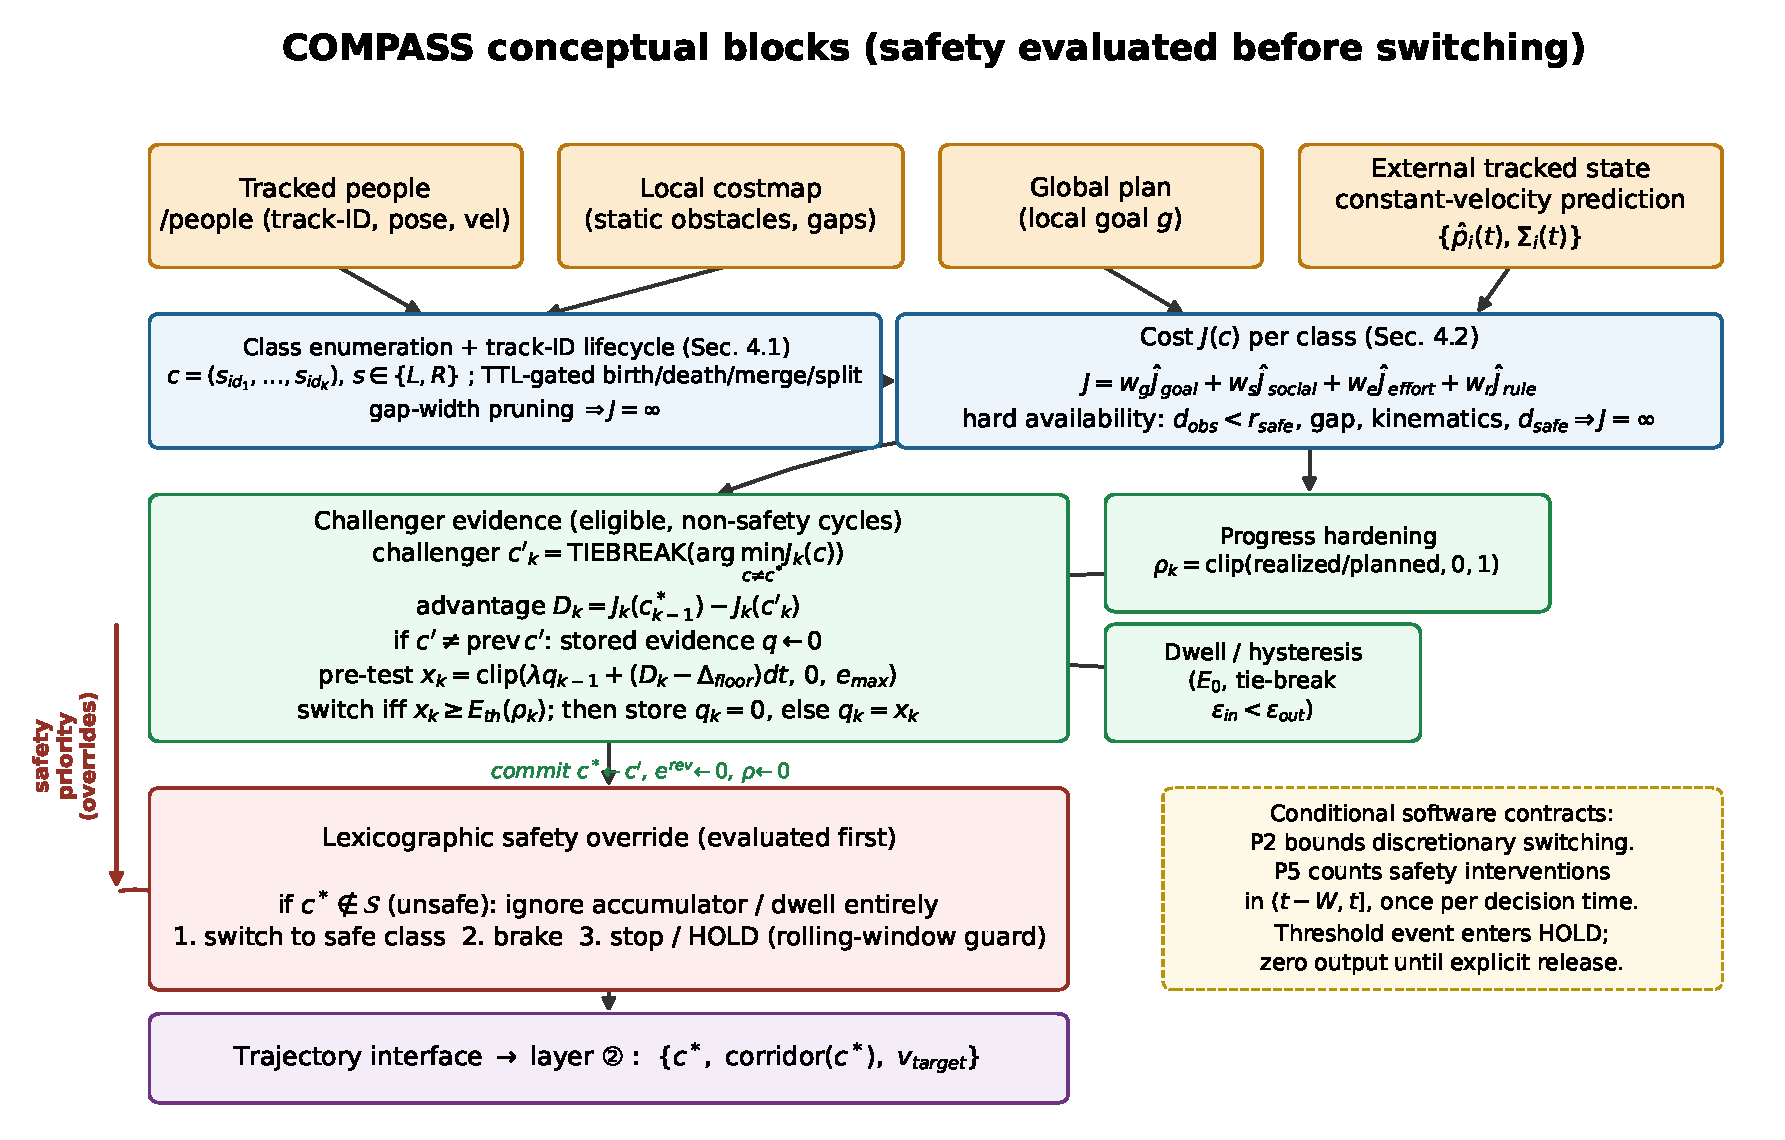
\includegraphics[width=\textwidth]{figures/fig_decision_flow.pdf}
\caption{Control-cycle flowchart of the COMPASS decision layer. Inputs (tracked people \code{/people}, local costmap, global plan, Kalman constant-velocity predictions) flow into track-ID-based class enumeration (\S4.1) and cost $J(c)$ computation (\S4.2), which feed the leaky-evidence-accumulation commitment switch based on the single-challenger accumulator $\Erev$ (\S4.3, \S4.5 stage 3), combined with dwell and progress hardening to decide whether to switch, over which the lexicographic safety override (\S4.4, \S4.5 stage 2) is layered with top priority. The yellow box at bottom right summarizes that the switching dynamics close through the single-challenger accumulator $\Erev$ alone, designed so that its reachable upper bound satisfies the two-sided condition $E_0 < \Eremax < E_0(1+k_\rho)$ (\S4.6).}
\label{fig:decisionflow}
\end{figure}

The implementation is a \code{nav2\_core::Controller} plugin (\code{compass\_nav2::CompassController}) for ROS2 \texttt{Nav2}~\cite{macenski2020nav2}, hosted by the \code{controller\_server}. One decision cycle executes per \code{computeVelocityCommands} call; the cycle rate is set by the \code{controller\_server}'s \code{controller\_frequency} parameter (20.0 Hz in the deployed configuration of this implementation); the costmap comes from \code{Costmap2DROS}, and human tracks are received via a subscription to \code{/people} (\code{compass\_msgs/People}). The plugin complies with the \texttt{Nav2} lifecycle contract (\code{configure}/\code{activate}/\code{deactivate}/\code{cleanup}), outputs \code{TwistStamped}, and maintains corresponding state (labels, $e$, $\rho$, TTL, $\text{prev}_{c'}$, safety dwell) across cycles.

\textbf{System interface of the decision layer.} Table~\ref{tab:interface} transcribes the interface contract directly from the implementation code.

\begin{table}[t]
\centering
\caption{System interface of the COMPASS decision layer, transcribed from the implementation code.}
\label{tab:interface}
\resizebox{\textwidth}{!}{%
\begin{tabular}{llllll}
\toprule
Interface & Format & Frame handling & Rate/timing & QoS & Freshness policy \\
\midrule
\code{/people} subscription & \code{compass\_msgs/People} & Message frame $\to$ costmap global frame via \code{tf2}; all people in a message dropped on transform failure & Async.\ receipt, latest value consumed at cycle start & \code{rclcpp::SensorDataQoS()} = best-effort $\cdot$ volatile $\cdot$ keep-last depth 5 & Last-value; no age cutoff; 0 people if absent \\
Costmap & \code{Costmap2DROS} (shared with \code{controller\_server}) & Costmap global frame & Synchronous, within cycle & --- & Governed by costmap's own update rate \\
Global plan & \code{nav\_msgs/Path} (\code{setPlan}) & Plan frame & Replaced on new plan & --- & Latest plan retained \\
Decision cycle & \code{computeVelocityCommands} call & --- & \code{controller\_frequency} (20.0 Hz); $dt$ = measured inter-call interval (0.1 s fallback on first cycle or non-advancing clock) & --- & --- \\
Output & \code{geometry\_msgs/TwistStamped} & Input pose frame & Once per call & --- & --- \\
\bottomrule
\end{tabular}%
}
\end{table}

Here $dt$ is not a fixed constant but the measured inter-call interval (distinct from the offline harness's fixed $dt=0.05$ s in \S5.1), and the absence of a message-age cutoff for \code{/people} is a fact of the implementation as-is --- the TTL of \S4.1 is the TTL of \Class\ identity, a separate mechanism from this. Meanwhile, end-to-end pipeline characteristics --- executor scheduling jitter, rmw/DDS queueing, TF delay, costmap update concurrency, \code{controller\_server} dispatch overhead, and the effect of input-freshness handling --- are not characterized in this paper; their measurement belongs to the planned evaluation (\S5.6).

\FloatBarrier
\subsection{Property analysis}

We state five properties as propositions. P1, P2, and P4 include proofs; P3 and P5 are argued. This paper formulates P1 as a probabilistic statement (a per-cycle upper bound on switching probability and rate) and P4 on the basis of $\rho$ dynamics, a lower bound on the lateral-progress rate, and the \textbf{containment of the reachable upper bound of the single-challenger accumulator}.

One point of scope is worth stating before the propositions rather than after them. The anti-oscillation guarantee this paper \textbf{carries in its headline claims is P2} (\S4.7): a deterministic lower bound of $N_{\min}(\rho) = \lceil \Eth(\rho)/((D_{\max}-\Dfloor)\,dt)\rceil$ control cycles on the interval between two consecutive discretionary switches, which holds on every sample path and assumes nothing about the distribution of $D_k$ beyond the range bound $D_k \le D_{\max}$. Two qualifications are stated with it rather than left implicit. First, the bound is informative only under the non-vacuity condition $E_0 > (D_{\max}-\Dfloor)\,dt$ ($N_{\min}(0) \ge 2$), which we declare as a design condition alongside \eqref{eq:twosided} (Remark~\ref{rem:p2nonvac}); without it P2 collapses to the one-cycle bound that every discrete-time policy satisfies. Second, P2 is an upper bound on the switching rate only --- a policy that never switches satisfies it --- so temporal consistency in the sense this paper intends is P2 \emph{together with} the response-time bound of Proposition~\ref{prop:p2live}, which guarantees that a sustained challenger advantage produces a discretionary switch within a finite, explicitly computable number of cycles. P1's exponential form (part (ii)) is a sharper statement --- it upgrades ``switching is infrequent'' to ``switching is exponentially rare'' --- but it is \emph{conditional on an independence hypothesis} on $\{D_k\}$ that stationarity alone does not supply, as Remark~\ref{rem:dep} shows by counterexample. We therefore state P1(ii) as a conditional refinement and rest the paper's temporal-consistency claim on P2.

\textbf{The single-challenger accumulator and notation (a premise for P4/\S4.9 consistency).} The switching dynamics of this paper close over the \textbf{single} leaky-evidence accumulator of \S4.3/\S4.5. Since this accumulator, by definition, always integrates the advantage evidence of the challenger $c'$ seeking to overturn the current commitment $c^*$, we denote it in the property analysis below as the \textbf{challenger accumulator} $\Erev$ --- it is \textbf{exactly the same single variable} as the accumulation equation of \S4.3 and the state variable $e$ of the \S4.5 algorithm; the superscript rev merely denotes the role ``evidence for a challenge that would reverse the current commitment'' and is not a separate accumulator. We write the maximum value $\Erev$ can reach as $\Eremax$ (the smaller of the leak equilibrium bound and the clip bound $e_{\max}$ when $\lambda < 1$; derived in P4).

The soundness of the switching dynamics is summarized by a single \textbf{two-sided condition} on the reachable upper bound of this single accumulator.
\begin{equation}
E_0 < \Eremax < E_0(1 + k_\rho)
\label{eq:twosided}
\end{equation}
The lower bound ($\Eremax > E_0$) is a \textbf{liveness} condition guaranteeing that discretionary switching is possible at all at $\rho = 0$ (\S4.9), and the upper bound ($\Eremax < E_0(1+k_\rho)$) is the \textbf{P4 containment} condition that once the maneuver is sufficiently progressed ($\rho > \bar\rho$; the boundary point itself belongs to the switching window, see Remark~\ref{rem:lockboundary}), challenge accumulation is trapped below the threshold and reversal is blocked. Since both requirements are a lower and upper bound on the same variable $\Eremax$, they can be satisfied simultaneously without contradiction. A third declared condition, $E_0 > (D_{\max}-\Dfloor)\,dt$ (P2 non-vacuity, Remark~\ref{rem:p2nonvac}), is independent of \eqref{eq:twosided}: it bounds the threshold from below by the largest single-cycle innovation rather than from above by the reachable bound. The self-contradiction of the previous formulation arose from imposing a separate ``above-threshold headroom'' requirement ($e_{\max} > E_0(1+k_\rho)$) on the same upper bound, which collides head-on with this containment upper bound; as discussed in \S4.9, we clarify that this headroom requirement was never itself a soundness condition and withdraw it.

\begin{proposition}[Anti-oscillation --- probabilistic form] \label{prop:p1}
Suppose the challenger advantage $D_k$ is a stationary stochastic process with mean 0, bounded variance $\mathrm{Var}[D_k] \le \sigma_D^2$, and \textbf{bounded range} $|D_k| \le D_{\max}$ almost surely, and let $0 < \Dfloor < D_{\max}$. Write $X_k := (D_k - \Dfloor)\,dt$ for the \textbf{driving innovation} of the accumulation recursion of \S4.3. Then (i) the innovation has strictly negative mean,
\begin{equation}
\mathbb{E}[X_k] = (\mathbb{E}[D_k] - \Dfloor)\,dt = -\Dfloor\, dt < 0,
\label{eq:innovdrift}
\end{equation}
so in ambiguous configurations (mean advantage 0) a discretionary switch requires the fluctuations of $D_k$ to overcome a persistent negative bias in the input. We emphasize that \eqref{eq:innovdrift} is a statement about the \emph{raw input} to the recursion, \textbf{not} about the one-cycle increment of the reflected state $\Erev_k$: the lower clip at $0$ truncates negative innovations, so the expected state increment $\mathbb{E}[\Erev_{k+1} - \Erev_k]$ can be strictly positive at the boundary even though $\mathbb{E}[X_k] < 0$ (Remark~\ref{rem:boundarydrift}). Rarity is therefore quantified below as a crossing-probability bound, not as a drift argument on the state.

Suppose further that $\{D_k\}$ is \textbf{i.i.d.}\ (the \textbf{independence hypothesis} of this proposition). If $\mathbb{P}(X_1 > 0) = 0$, the accumulator never leaves $0$ and the discretionary switching probability is exactly $0$. Otherwise, boundedness of $X_1$ together with $\mathbb{E}[X_1] < 0$ implies that the \textbf{Lundberg equation} $\mathbb{E}[e^{\theta X_1}] = 1$ has a unique positive root $\theta^* > 0$ (the adjustment coefficient), and (ii) the per-cycle switching probability admits the uniform bound
\begin{equation}
\mathbb{P}\big(\Erev_k \ge E_0\big) \;\le\; e^{-\theta^* E_0} \qquad \text{for every cycle } k,
\label{eq:pswitch}
\end{equation}
whence the expected number of discretionary switches in any window of $N$ cycles is at most $N e^{-\theta^* E_0}$, and the expected switching rate per unit time is at most $(1/dt)\, e^{-\theta^* E_0}$ --- both exponentially small in $E_0$, with an exponent $\theta^*$ that is increasing in the margin $\Dfloor$. The bound \eqref{eq:pswitch} is a \emph{marginal, per-cycle} bound: over an unbounded horizon of persistent ambiguity an eventual crossing is not excluded (nor should it be --- the liveness condition of \S4.9 requires the threshold to be reachable); what is guaranteed is that crossings are exponentially rare per cycle.

Part (ii) is \emph{conditional on the independence hypothesis and is not established under stationarity alone}; see Remark~\ref{rem:dep} for a counterexample. Accordingly the guarantee this paper carries in its headline claims is the \emph{deterministic} switching-rate bound P2 (\S4.7), which requires no distributional hypothesis on $D_k$ beyond the range bound; P1(ii) is a refinement that sharpens rarity from ``bounded frequency'' to ``exponentially rare'' when the independence hypothesis holds. Extension to dependent inputs is discussed --- and deliberately \emph{not} claimed as a theorem --- in Remark~\ref{rem:iid}.
\end{proposition}

\begin{remark}[Sign of the state increment at the reflecting boundary] \label{rem:boundarydrift}
The distinction drawn in part (i) is not pedantic; an earlier formulation of this proposition called \eqref{eq:innovdrift} ``the one-cycle expected increment of the challenger accumulator,'' and that reading is false under the proposition's own hypotheses. Take $D_k$ i.i.d.\ uniform on $\{-a, +a\}$ with $\Dfloor < a \le D_{\max}$, and start at the boundary $\Erev_0 = 0$. Then $\Erev_1 = \mathrm{clip}(X_1, 0, e_{\max})$, so (for $(a-\Dfloor)dt \le e_{\max}$)
\begin{equation}
\mathbb{E}[\Erev_1 - \Erev_0] = \tfrac{1}{2}(a - \Dfloor)\,dt \;>\; 0,
\end{equation}
even though $\mathbb{E}[X_1] = -\Dfloor\,dt < 0$: reflection truncates the negative half of the innovation and keeps the positive half. A negative-mean input therefore does \emph{not} make the reflected state a supermartingale, and no drift argument on the state can carry part (ii). This is the standard situation of queueing theory --- a stable queue has negative-mean net input yet strictly positive expected growth from empty --- and it is why the proof below routes through a pathwise domination by an unreflected random walk and a maximal inequality, rather than through the state's expected increment.
\end{remark}

\begin{remark}[On the boundedness hypothesis]
The range hypothesis $|D_k| \le D_{\max}$ is not an additional restriction on the system: by the $[0,1]$ normalization of \S4.2 the cost $J = \sum_X w_X \hat J_X$ is bounded, so the advantage $D_k = J_k(c^*_{k-1}) - J_k(c'_k)$ of \S4.3 is bounded by construction, and $D_k \le D_{\max}$ is the same hypothesis already carried by P2 (\S4.7), P4 (\S4.8), and the reachable bound $\Eremax$ (\S4.8). It is nevertheless stated \emph{explicitly} here, because part (ii) is an exponential bound and an exponential bound requires a finite exponential moment, which stationarity, zero mean, and finite variance do not supply on their own. A centred Student-$t_3$ advantage, for instance, satisfies every one of those three conditions yet has a polynomially decaying tail and no finite moment generating function, so no adjustment coefficient exists for it and a bound of the form \eqref{eq:pswitch} cannot hold. Under $|D_k| \le D_{\max}$ this failure mode is excluded, and the normalization of \S4.2 guarantees the hypothesis holds for the object this paper actually constructs.
\end{remark}

\begin{remark}[Why stationarity alone is not enough] \label{rem:dep}
Stationarity, zero mean, bounded variance and bounded range together are still not enough for part (ii), and it is worth being explicit about why, because the gap is not a technicality of the proof method but a genuine failure of the conclusion.

Draw $Z \in \{-a, +a\}$ once, with probability $1/2$ each and $\Dfloor < a \le D_{\max}$, and set $D_k = Z$ for every $k$. The joint law of $(D_{k+1}, \dots, D_{k+n})$ does not depend on $k$, so $\{D_k\}$ is strictly stationary; it has mean 0, variance $a^2$, and range bounded by $D_{\max}$. Yet on the branch $Z = +a$ every increment equals $(a - \Dfloor)dt > 0$, so $\Erev$ rises monotonically and crosses \emph{any} threshold $E_0 < \Eremax$ within $\lceil E_0/((a-\Dfloor)dt)\rceil$ cycles, while on the branch $Z = -a$ it never leaves $0$. Hence $P_{\text{switch}} \to 1/2$ as the horizon grows, with \emph{no} decay in $E_0$ whatsoever --- the exponential bound \eqref{eq:pswitch} fails by an arbitrarily large factor.

The mechanism is that a single draw persisting forever is perfectly admissible under stationarity, and no amount of bounded support repairs it: the process never forgets its regime, so no argument that needs fresh randomness --- independent increments, or independent blocks --- has anything to work with. This is precisely the failure mode the i.i.d.\ hypothesis of part (ii) excludes, and any relaxation of that hypothesis would have to exclude it too (Remark~\ref{rem:iid}). Note also that this counterexample says nothing about P2 (\S4.7), whose inter-switch interval bound is deterministic and holds on every sample path, including the adversarial one just constructed --- which is why P2, not P1(ii), carries the headline guarantee.
\end{remark}

\begin{proof}
Throughout, $\{D_k\}$ is i.i.d.\ with the moment and range hypotheses of the statement, and $X_k = (D_k - \Dfloor)\,dt$. Part (i) is the one-line computation \eqref{eq:innovdrift}; Remark~\ref{rem:boundarydrift} explains why it must be read as a statement about the input, not about the state. Note first that the lower clip is a \textbf{reflecting (saturating)} boundary, not an absorbing one: $\Erev$ is held at $0$ only while the update would go non-positive, and leaves $0$ on the first sufficiently positive innovation, so negative input drift does not trap the process at $0$ --- which is exactly why the earlier ``expected hitting time'' framings were uninformative, and why part (ii) is stated as a per-cycle probability bound whose \emph{scaling} in $E_0$ is the design-relevant quantity. We prove part (ii) in three steps; the trivial case $\mathbb{P}(X_1 > 0) = 0$ was dispatched in the statement.

\emph{Step 1 (pathwise domination).} Define the \textbf{Lindley recursion} \cite{lindley1952queue} driven by the same innovations, $W_0 = 0$, $W_k = \max(W_{k-1} + X_k,\, 0)$: the leak-free ($\lambda = 1$), unclipped-above, never-reset companion of the recursion of \S4.3. We claim $\Erev_k \le W_k$ for every $k$, on every sample path. Induction: $\Erev_0 = W_0 = 0$ (a discretionary switch requires a challenge to accumulate from the post-switch or post-retarget reset, both of which set $e = 0$). Suppose $\Erev_{k-1} \le W_{k-1}$. If cycle $k$ is a normal update, then since $\lambda \le 1$ and $\Erev_{k-1} \ge 0$,
\[
\Erev_k = \mathrm{clip}(\lambda \Erev_{k-1} + X_k,\, 0,\, e_{\max}) \le \max(\Erev_{k-1} + X_k,\, 0) \le \max(W_{k-1} + X_k,\, 0) = W_k;
\]
if cycle $k$ resets the accumulator (a switch fired, or the challenge target changed), then $\Erev_k = 0 \le W_k$. The leak, the upper clip, and every reset can only \emph{lower} the state, so the implemented accumulator is dominated pathwise by the Lindley walk.

\emph{Step 2 (adjustment coefficient and maximal inequality).} Unfolding the Lindley recursion gives the suffix-sum representation $W_k = \max_{0 \le j \le k} (X_k + X_{k-1} + \cdots + X_{k-j+1})$ (empty sum $= 0$), and since the $X_i$ are i.i.d., reversing the order of the increments shows that $W_k$ has, for each fixed $k$, the same distribution as $\max_{0 \le j \le k} S_j$ with $S_j = X_1 + \cdots + X_j$. Let $\psi(\theta) = \log \mathbb{E}[e^{\theta X_1}]$: it is finite for all $\theta$ (bounded range), convex, with $\psi(0) = 0$ and $\psi'(0) = \mathbb{E}[X_1] = -\Dfloor\,dt < 0$; and since $\mathbb{P}(X_1 > 0) > 0$, $\psi(\theta) \to \infty$ as $\theta \to \infty$. Hence $\psi$ has a unique positive root $\theta^*$, i.e., $\mathbb{E}[e^{\theta^* X_1}] = 1$. Then $M_j = e^{\theta^* S_j}$ is a nonnegative martingale with $M_0 = 1$, and the maximal inequality for nonnegative supermartingales (Ville's inequality) gives
\[
\mathbb{P}\Big(\sup_{j \ge 0} S_j \ge E_0\Big) = \mathbb{P}\Big(\sup_{j \ge 0} M_j \ge e^{\theta^* E_0}\Big) \le e^{-\theta^* E_0}.
\]
This is Kingman's bound on the waiting time of a single-server queue \cite{kingman1970queues}, specialized to our increments; it enters as a theorem, not an analogy. (Under zero mean and finite variance alone no root $\theta^*$ need exist; see the remark on the boundedness hypothesis above. The i.i.d.\ hypothesis is consumed twice in this step --- once for the reversal identity, once for the martingale property --- and neither survives bare stationarity, per Remark~\ref{rem:dep}.)

\emph{Step 3 (from crossing to switching).} A discretionary switch at cycle $k$ requires $\Erev_k \ge \Eth(\rho_k) \ge E_0$ (progress hardening only raises the threshold). By Steps 1--2, for every $k$,
\[
\mathbb{P}(\text{switch at cycle } k) \le \mathbb{P}(\Erev_k \ge E_0) \le \mathbb{P}(W_k \ge E_0) = \mathbb{P}\Big(\max_{0 \le j \le k} S_j \ge E_0\Big) \le e^{-\theta^* E_0},
\]
which is \eqref{eq:pswitch}. Linearity of expectation then bounds the expected number of discretionary switches in any $N$-cycle window by $N e^{-\theta^* E_0}$, i.e., the expected switching rate per unit time by $(1/dt)\, e^{-\theta^* E_0}$. Monotonicity of $\theta^*$ in the margin follows from $\psi$ decreasing pointwise (for $\theta > 0$) as $\Dfloor$ grows. Finally, since the leak and the resets were absorbed in Step 1, the bound holds verbatim for every $\lambda \le 1$; a smaller $\lambda$ only widens the gap between the implemented process and the dominating walk, so in practice the true switching probability is further below the bound.

Thus the extreme-cycle oscillation that memoryless argmin exhibits near a symmetric point is \textbf{probabilistically} suppressed: in ambiguous configurations a discretionary switch occurs in any given cycle only with exponentially small probability, when the fluctuations of $D_k$ have accumulated enough to push the evidence over the threshold.
\end{proof}

\begin{remark}[Tuning guidance: a closed-form approximation of $\theta^*$] \label{rem:tuning}
The exact adjustment coefficient $\theta^*$ of Proposition~\ref{prop:p1} depends on the full law of $D_1$ through the Lundberg equation $\mathbb{E}[e^{\theta (D_1-\Dfloor)dt}] = 1$; boundedness and variance alone do not determine it. For parameter tuning it is nevertheless useful to have a closed form. Expanding the log-moment-generating function to second order, $\psi(\theta) \approx -\theta\,\Dfloor\,dt + \tfrac{1}{2}\theta^2 \sigma_D^2\, dt^2$, and solving $\psi(\theta) = 0$ gives the \textbf{small-drift, quasi-Gaussian approximation}
\begin{equation}
\theta^* \approx \frac{2\Dfloor}{\sigma_D^2\, dt},
\qquad\text{whence}\qquad
r_{\text{switch}} \lesssim \frac{1}{dt} \exp\!\left(-\frac{2\Dfloor E_0}{\sigma_D^2\, dt}\right).
\label{eq:thetaapprox}
\end{equation}
We use \eqref{eq:thetaapprox} \emph{only} as design guidance --- it indicates how rarity scales as the margin $\Dfloor$ or the threshold $E_0$ grows, the variance $\sigma_D^2$ shrinks, or the cycle time $dt$ shortens --- and it is \textbf{not} the coefficient the guarantee is stated with: the guarantee \eqref{eq:pswitch} carries the exact root $\theta^*$. The variance scale in \eqref{eq:thetaapprox} is matched to the \textbf{per-cycle increment variance $\sigma_D^2\,dt^2$} (equivalently, the per-unit-time variance $\sigma_D^2\,dt$), which restores the $1/dt$ factor in $\theta^*$ and in the switching-rate bound that an unnormalized reading would drop.
\end{remark}

\begin{remark}[Deterministic special case]
If $|D_k| \le \Dfloor$ for all $k$, the increment is always $\le 0$, so $\Erev_k \equiv 0$ and the switching probability is exactly 0 --- this is the trivial case $\mathbb{P}(X_1 > 0) = 0$ of Proposition~\ref{prop:p1}(ii), and the statement of the initial deterministic formulation. This probabilistic form relaxes that strong assumption --- from ``every realization is inside the margin'' to ``mean 0, bounded variance, and range bounded by $D_{\max}$'' --- and as $\sigma_D^2 \to 0$ in the tuning approximation \eqref{eq:thetaapprox} the bound tends to 0, continuously recovering the deterministic case. Note that only the pointwise margin condition $|D_k| \le \Dfloor$ is relaxed; the range bound $|D_k| \le D_{\max}$, being a structural consequence of the cost normalization rather than an assumption about the environment, is retained.
\end{remark}

\begin{remark}[IID hypothesis and autocorrelation] \label{rem:iid}
Proposition~\ref{prop:p1}(ii) is stated and proved for i.i.d.\ $D_k$. The $D_k$ of this paper, however, is a stationary process that allows autocorrelation due to the temporal correlation of human motion and prediction, and we are explicit about what is and is not claimed across that gap. A natural route to a dependent version exists --- under geometric $\alpha$-mixing one would decompose the trajectory into regenerative blocks, whose finite exponential moments the range hypothesis $|D_k| \le D_{\max}$ supplies, and re-run the Step-2 argument on block sums --- but turning that route into a theorem requires quantified hypotheses (an explicit regeneration structure, a mixing rate, and a dependence-adjusted adjustment coefficient) that this paper does not formalize, so \textbf{no exponential bound is claimed here for dependent inputs}. Earlier versions offered a fallback in which $\theta^*$, or the effective variance replacing $\sigma_D^2$, was read as ``absorbing the autocorrelation structure'' --- with the long-run variance $\sum_k \mathrm{Cov}(D_0, D_k)$ substituted for the marginal variance --- while claiming only the qualitative form ``exponential decay in $\Dfloor \cdot E_0$.'' That fallback is withdrawn: a long-run variance does not determine a large-deviation rate, no theorem connects it to the first-passage behaviour of this reflected recursion, and Remark~\ref{rem:dep} exhibits a stationary process for which the qualitative form itself is false. Where independence cannot be asserted, the guarantee available is P2 (\S4.7), which is deterministic, pathwise, and indifferent to the dependence structure. Whether approximate independence is defensible for a given deployment is an empirical question, and estimating the autocorrelation structure of $D_k$ from logged encounters is a measurement target of \S5.5 and the planned evaluation (\S5.6). Finally, the leak requires no separate treatment: Step 1 of the proof absorbs every $\lambda \le 1$, so introducing $\lambda < 1$ leaves the bound \eqref{eq:pswitch} valid verbatim --- it only widens the gap between the implemented process and the dominating walk.
\end{remark}

\begin{remark}[$\lambda \cdot \Eth$ interaction]
The interaction of $\lambda$ and $\Eth$ (the leak makes reaching the threshold depend not on the simple integral of $D$ but on its temporal \textbf{shape} --- a short, strong advantage pulse accumulates before leaking away and easily crosses the threshold, whereas a long, weak advantage is offset by leaking and falls short of the threshold) is further analyzed in \S4.9.
\end{remark}

\begin{proposition}[Switching-rate bound] \label{prop:p2}
If the challenger advantage is bounded, $D_k \le D_{\max}$ with $D_{\max} > \Dfloor$, then between two consecutive discretionary switches at least
\begin{equation}
N_{\min}(\rho) \;=\; \left\lceil \frac{\Eth(\rho)}{(D_{\max}-\Dfloor)\,dt} \right\rceil
\label{eq:nmin}
\end{equation}
control cycles elapse; equivalently $\Delta t_{\text{switch}} \ge N_{\min}(\rho)\,dt \ge \Eth(\rho)/(D_{\max}-\Dfloor)$. At $\rho = 0$, $\Eth(0) = E_0$; at $\rho > 0$, progress hardening gives $\Eth(\rho) = E_0(1+k_\rho \rho^p) \ge E_0$, so the bound \textbf{grows} with progress (reversal becomes harder as the maneuver progresses). The bound is informative only when $N_{\min}(0) \ge 2$, i.e.
\begin{equation}
E_0 \;>\; (D_{\max}-\Dfloor)\,dt
\label{eq:p2nonvac}
\end{equation}
(the accumulator cannot cross the $\rho = 0$ threshold within a single cycle); when \eqref{eq:p2nonvac} fails, $N_{\min}(0) = 1$ and P2 asserts nothing beyond what sampling already imposes. We adopt \eqref{eq:p2nonvac} as a declared design condition alongside \eqref{eq:twosided}.
\end{proposition}

\begin{proof}
Immediately after a discretionary switch the accumulator is reset, $\Erev = 0$. In every subsequent cycle the pre-clip update satisfies $\lambda\Erev_{k-1} + (D_k-\Dfloor)\,dt \le \Erev_{k-1} + (D_{\max}-\Dfloor)\,dt$ because $\lambda \le 1$, and $\mathrm{clip}(\cdot,0,e_{\max})$ never increases its argument; hence after $n$ cycles $\Erev \le n\,(D_{\max}-\Dfloor)\,dt$. A discretionary switch requires $\Erev \ge \Eth(\rho)$, which forces $n \ge \Eth(\rho)/((D_{\max}-\Dfloor)\,dt)$, and since $n$ is an integer, $n \ge N_{\min}(\rho)$. The leak and the upper clip can only delay or block threshold attainment, never advance it, so the bound holds for every $\lambda \le 1$ and every $e_{\max}$ (the headroom-withdrawal argument of \S4.9). Hence the switching frequency is bounded above by $1/(N_{\min}\,dt)$ on every sample path, and behavior is legible. (Whereas P1(ii) guarantees the \textbf{exponential rarity} of switching in ambiguous configurations only under its independence hypothesis, P2 deterministically guarantees an \textbf{upper bound on switching frequency} in arbitrary configurations, on every sample path and with no distributional hypothesis --- which is why P2 is the guarantee this paper claims. The bound holds in particular on the stationary counterexample of Remark~\ref{rem:dep}, where P1(ii) does not. It is an upper bound on the rate only: a policy that never switches satisfies it, and the complementary lower bound on responsiveness is Proposition~\ref{prop:p2live}. Note that, per the drift analysis of \S4.2, the $\Dfloor$ in this bound has a meaning that is constant across cycles only when the normalization constants are fixed as pre-calibrated constants.)
\end{proof}

\begin{remark}[Non-vacuity of P2 and the default knobs] \label{rem:p2nonvac}
Condition \eqref{eq:p2nonvac} is not implied by the two-sided condition \eqref{eq:twosided}, and the boundary instance of Remark~\ref{rem:lockboundary} shows the difference: with $dt = 0.05$, $\Dfloor = 0.05$, $D_{\max} = 0.95$ and $E_0 = 0.03$, \eqref{eq:twosided} holds but $(D_{\max}-\Dfloor)\,dt = 0.045 > E_0$, so $N_{\min}(0) = 1$ and P2 is vacuous there: an advantage sequence that takes the value $D_{\max}$ against whichever \Class\ is currently committed drives $\Erev$ from $0$ to $0.045 \ge E_0$ in one cycle after every reset and flips the class every cycle while satisfying the bound exactly. That instance is retained only to exhibit the boundary of the lock region; it is not an admissible operating point once \eqref{eq:p2nonvac} is imposed. For the default knobs of Table~\ref{tab:params} the condition holds with margin. By the $[0,1]$ normalization of \S4.2, $D_k = J_k(c^*_{k-1}) - J_k(c'_k)$ satisfies $|D_k| \le \sum_X w_X = 2.8$ for the default weights, so in the worst case $(D_{\max}-\Dfloor)\,dt = 0.1375 < E_0 = 0.30$ and $N_{\min}(0) = 3$ cycles ($0.15$ s); if the realized advantage is bounded by a single normalized term, $D_{\max} \le 1$, then $N_{\min}(0) = 7$ cycles ($0.35$ s), and for $D_{\max} \le 0.5$, $N_{\min}(0) = 14$ cycles ($0.70$ s). Progress hardening multiplies each of these by $(1 + k_\rho \rho^p)$. The worst-case figure is reported deliberately: P2 is a weak guarantee when the advantage can saturate every cost term at once, and the practical content of temporal consistency at the default knobs rests on the response-time bound below and, for i.i.d.\ inputs, on P1(ii).
\end{remark}

\begin{proposition}[Response-time bound under a sustained advantage] \label{prop:p2live}
Fix a challenger $c'$ and a cycle $k_0$ with $\Erev_{k_0} \ge 0$. Suppose that for all $k > k_0$ no safety intervention occurs, the challenge target does not change, and the advantage is sustained, $D_k \ge D_{\text{sus}}$ with $D_{\text{sus}} > \Dfloor$; write $a = (D_{\text{sus}}-\Dfloor)\,dt$ and let $\bar E$ be an upper bound on $\Eth(\rho_k)$ over the cycles considered (for instance $\bar E = \Eth(\hat\rho)$ when $\rho_k \le \hat\rho$ on that window). If $e_{\max} \ge \bar E$ and either $\lambda = 1$ or $a/(1-\lambda) > \bar E$, then a discretionary switch fires within
\begin{equation}
N_{\text{resp}} \;=\; \left\lceil \frac{\ln\!\big(1 - \bar E\,(1-\lambda)/a\big)}{\ln \lambda} \right\rceil \quad (\lambda < 1), \qquad N_{\text{resp}} = \left\lceil \bar E / a \right\rceil \quad (\lambda = 1)
\label{eq:nresp}
\end{equation}
cycles after $k_0$. Conversely, if $\Erev_{k_0} < \underline{E}$ and $D_k \le \bar D$ for all $k > k_0$ with $\lambda < 1$ and $(\bar D-\Dfloor)\,dt/(1-\lambda) \le \underline{E} \le \Eth(\rho_k)$ on the window, then $\Erev_k < \underline{E}$ throughout and no discretionary switch fires: a bounded advantage whose leak equilibrium lies below the threshold can never produce a switch.
\end{proposition}

\begin{proof}
Let $\tilde e_n = a(1-\lambda^n)/(1-\lambda)$ for $\lambda < 1$ (and $\tilde e_n = n a$ for $\lambda = 1$) be the trajectory of the unclipped recursion driven from $0$ by the constant increment $a$; it is increasing in $n$ and converges to $a/(1-\lambda)$. Under the stated equilibrium condition there is a least $n^*$ with $\tilde e_{n^*} \ge \bar E$, and solving $\lambda^n \le 1 - \bar E(1-\lambda)/a$ gives $n^* = N_{\text{resp}}$. We claim $\Erev_{k_0+n} \ge \tilde e_n$ for every $n < n^*$ at which no switch has yet fired. For $n = 0$ this is $\Erev_{k_0} \ge 0$. If it holds at $n-1$, then because $(D_k - \Dfloor)\,dt \ge a$ and $x \mapsto \mathrm{clip}(\lambda x + (D_k-\Dfloor)\,dt,\,0,\,e_{\max})$ is nondecreasing in $x$, $\Erev_{k_0+n} \ge \mathrm{clip}(\lambda \tilde e_{n-1} + a,\,0,\,e_{\max}) = \min(e_{\max}, \tilde e_n) = \tilde e_n$, using $\tilde e_n < \bar E \le e_{\max}$ for $n < n^*$. At $n = n^*$ the same step gives $\Erev_{k_0+n^*} \ge \min(e_{\max}, \tilde e_{n^*}) \ge \bar E \ge \Eth(\rho_{k_0+n^*})$, so the switching rule of \S4.4 ($\Erev_k \ge \Eth(\rho_k)$, non-strict) fires at or before cycle $k_0+n^*$; by hypothesis nothing other than a discretionary switch resets the accumulator on the window. For the converse, the same monotonicity in the other direction gives $\Erev_{k_0+n} \le \lambda^n \Erev_{k_0} + (1-\lambda^n)(\bar D-\Dfloor)\,dt/(1-\lambda) < \lambda^n \underline{E} + (1-\lambda^n)\underline{E} = \underline{E} \le \Eth(\rho_{k_0+n})$ for every $n \ge 1$, so the rule never fires.
\end{proof}

\begin{remark}[Response time at the default knobs] \label{rem:resptime}
With $dt = 0.05$, $\Dfloor = 0.05$, $E_0 = 0.30$, $\lambda = 0.97$ and $k_\rho = 1$, a discretionary switch at $\rho = 0$ is reachable only for a sustained advantage exceeding $\Dfloor + E_0(1-\lambda)/dt = 0.23$, and at $\rho = 1$ only above $\Dfloor + E_0(1+k_\rho)(1-\lambda)/dt = 0.41$. At $\rho = 0$, \eqref{eq:nresp} gives $N_{\text{resp}} = 76$ cycles ($3.8$ s) for $D_{\text{sus}} = 0.25$, $24$ cycles ($1.2$ s) for $0.40$, $17$ cycles ($0.85$ s) for $0.5$, and $7$ cycles ($0.35$ s) for $1.0$ --- the last coinciding with $N_{\min}(0)$ for $D_{\max} = 1$, as it must. These figures are consequences of the recursion, not measurements; \S5.3 compares them with the harness findings.
\end{remark}

\begin{proposition}[Safety dominance] \label{prop:p3}
In any cycle in which $c^* \notin \mathcal{S}$, the safety ladder fires regardless of accumulator state or progress.
\end{proposition}

\begin{proof}[Argument]
Because stage 2 (safety) of the algorithm is evaluated before stage 3 (discretionary) with lexicographic priority, commitment inertia can never delay the safety response in any case when a safety violation occurs. The safety-branch hysteresis of \S4.4 does not delay the safety \textbf{response itself}; it only determinizes the form of the response as a monotone descent of ``decelerate $\to$ stop'' rather than ``chattering at the switch stage.''
\end{proof}

\begin{proposition}[Maneuver completion --- $\rho$ dynamics and containment of the challenger accumulator] \label{prop:p4}
Suppose there is no safety intervention, the challenger advantage is bounded ($D_k \le D_{\max}$), the trajectory layer realizes the commanded cross-track progress rate at at least $v_{\text{lat,min}} > 0$ as in Assumption 3(d), and the cumulative disturbance retreat is bounded, $\sum_k b_k \le B < L_{\text{plan}}$ (the quantity used in the proof below). Then containment is \emph{pointwise}: in every cycle whose progress $\rho$ \textbf{strictly exceeds} the containment threshold $\bar\rho$ (derived below), reversal to the opposite \Class\ is blocked. If, moreover, $\rho$ never returns to or below $\bar\rho$ after first exceeding it (forward invariance; Remark~\ref{rem:nonmono}), the maneuver completes without reversal within at most $(L_{\text{plan}}+B)/(v_{\text{lat,min}}\, dt)$ cycles. In the pre-lock region ($\rho \le \bar\rho$), a sustained challenger advantage can still cross $\Eth(\rho)$ and trigger a discretionary switch --- this is not a defect but a legitimate switching window intentionally left open by the liveness lower bound $\Eremax > E_0$ (e.g., the one legitimate switch per encounter measured in \code{clean\_commit} in \S5.3), in which case the algorithm restarts with $\Erev \leftarrow 0 \cdot \rho \leftarrow 0$, and this guarantee applies identically to the new commitment. That is, what P4 excludes is reversal in the locked region ($\rho > \bar\rho$; the completion clause additionally requires the forward invariance stated above).
\end{proposition}

\begin{proof}
First we define the dynamics of $\rho$. Let progress be $\rho_k = \mathrm{clip}(L_{\text{real},k}/L_{\text{plan}}, 0, 1)$, where $L_{\text{real},k}$ is the cumulative realized cross-track progress and $L_{\text{plan}} = |\text{planned lateral offset of } c^*|$. The one-cycle realized progress is $\Delta L_k = v_{\text{lat},k} \cdot dt$, and by assumption $v_{\text{lat},k} \ge v_{\text{lat,min}}$ (per Assumption 3(d), $v_{\text{lat},k}$ is not the vehicle's lateral body-frame velocity but the progress rate along the cross-track coordinate, realized in non-holonomic drives as the product of forward speed and steering). However, since $\rho$ can stagnate or decrease if the robot is pushed by environmental change or the corridor narrows, we \textbf{do not assume monotone increase} and instead use a lower bound on the non-negative net increment. Letting $b_k \ge 0$ denote retreat due to disturbance ($b_k$ covers the \textbf{non-negative decrement of net progress} due to disturbance --- it collects all unplanned retreats that erode cross-track progress, such as being pushed, corridor narrowing, or momentary reversal, into a single non-negative term), $L_{\text{real},k} = L_{\text{real},k-1} + v_{\text{lat},k} dt - b_k$. Under the condition that the disturbance is bounded ($\sum_k b_k \le B < L_{\text{plan}}$, i.e., cumulative retreat does not consume the entire planned displacement), the lower bound on net progress is
\begin{equation}
L_{\text{real},K} \ge K \cdot v_{\text{lat,min}} \cdot dt - B,
\end{equation}
so after $K \ge (L_{\text{plan}} + B)/(v_{\text{lat,min}} \cdot dt)$ cycles, $L_{\text{real},K} \ge L_{\text{plan}}$, i.e., $\rho \to 1$ is reached.

Meanwhile, for locking (blocking reversal to the opposite \Class) to hold, the progress-hardening threshold $\Eth(\rho) = E_0(1+k_\rho \rho^p)$ must exceed the \textbf{maximum value reachable by the challenger accumulator $\Erev$}. The challenger accumulator increases by at most $(D_{\max}-\Dfloor)dt$ per cycle, decreases via the leak $\lambda$, and is clipped at $e_{\max}$. Hence, under $\lambda < 1$ (leak present), the reachable maximum of the challenger accumulator is the smaller of the leak-integral equilibrium bound and the clip bound, namely
\begin{equation}
\Eremax = \min\!\left(e_{\max},\ \frac{(D_{\max}-\Dfloor)\, dt}{1-\lambda}\right)
\label{eq:eremax}
\end{equation}
(the geometric series $\sum_{j\ge0} \lambda^j (D_{\max}-\Dfloor)dt = (D_{\max}-\Dfloor)dt/(1-\lambda)$ is the leak equilibrium bound, and the clip further caps it at $e_{\max}$). Only under the pure-integrator assumption $\lambda = 1$ does the leak-equilibrium term diverge to infinity, so that the reachable bound simplifies to the clip bound $e_{\max}$. Below, for generality, we write $\Eremax$ as the reachable bound. The \textbf{containment condition} is thus
\begin{equation}
\Eth(\rho) = E_0(1+k_\rho \rho^p) > \Eremax \qquad \text{(P4 containment condition at progress $\rho$)}
\end{equation}
and the boundary value at which the corresponding \emph{equality} $\Eth(\bar\rho) = \Eremax$ holds is
\begin{equation}
\bar\rho = \left(\frac{\Eremax/E_0 - 1}{k_\rho}\right)^{1/p}
\end{equation}
Since $\Eth$ is strictly increasing in $\rho$ (for $k_\rho > 0$, $p \ge 1$), the containment condition holds \textbf{exactly on the open region $\rho > \bar\rho$}; the boundary point $\rho = \bar\rho$ belongs to the switching window whenever $\Eremax$ is attained (Remark~\ref{rem:lockboundary}). The \textbf{existence condition} for a nonempty lock region $(\bar\rho, 1]$ is $\bar\rho < 1$ with $\bar\rho > 0$, i.e., $E_0 < \Eremax < E_0(1+k_\rho)$.

\textbf{Non-vacuity of containment.} Note that the lower bound $\Eremax > E_0$ in the above existence condition is \textbf{effectively equivalent to ``whether discretionary switching is possible at all.''} If the reachable bound $\Eremax$ of the challenger accumulator is below $E_0$, then $\Erev$ cannot even reach the threshold $\Eth(0) = E_0$ at $\rho=0$, so \textbf{no discretionary switch can ever occur}, and consequently the entire switching dynamics addressed by P1 and P2 becomes inert. That is, even though containment holds (since nothing ever switches), it is not ``the maneuver was locked'' but rather a degeneracy of ``there was never any switching capability to begin with,'' and the guarantee loses its meaning. The designer must therefore preserve a region of $(\lambda, \Eremax)$ that \textbf{simultaneously} satisfies containment (upper bound $\Eremax < E_0(1+k_\rho)$) and switchability (lower bound $\Eremax > E_0$); concrete guidance for this is given in the knob tuning of \S5.5.

Combined with the non-vacuity lower bound above, this containment condition organizes into the two-sided condition $E_0 < \Eremax < E_0(1+k_\rho)$ stated at the start of \S4.6 --- the lower bound is switching liveness at $\rho = 0$, and the upper bound is the existence of a nonempty lock region ($\bar\rho < 1$). Since both are a lower and upper bound on the same variable $\Eremax$, they can be satisfied simultaneously; the separate ``above-threshold headroom'' requirement ($e_{\max} > E_0(1+k_\rho)$) that produced the self-contradiction in the previous formulation is withdrawn and re-derived in \S4.9. Design is done by adjusting the leak-equilibrium term (via $\lambda$) and the clip bound $e_{\max}$ so as to place $\Eremax$ in the open interval $(E_0, E_0(1+k_\rho))$, ensuring that a nonempty lock region $(\bar\rho, 1]$ exists (design guidance is given in the knob tuning of \S5.5).

Once $\rho$ lies in the lock region ($\bar\rho < \rho \le 1$), switching to the opposite \Class\ is blocked; provided $\rho$ does not retreat to or below $\bar\rho$ thereafter (Remark~\ref{rem:nonmono}), $\rho$ reaches 1 along the lower bound above, and the maneuver completes; the number of cycles to completion is finitely bounded by $K \le (L_{\text{plan}}+B)/(v_{\text{lat,min}} \cdot dt)$.
\end{proof}

\begin{remark}[Boundary of the lock region] \label{rem:lockboundary}
The lock region is open at $\bar\rho$ by necessity, not by convention. When the clip binds ($e_{\max} \le (D_{\max}-\Dfloor)dt/(1-\lambda)$, so that $\Eremax = e_{\max}$ is \emph{attained}), the boundary case is realizable: take $dt = 0.05$, $\Dfloor = 0.05$, $D_{\max} = 0.95$, $\lambda = 0.5$, $E_0 = 0.03$, $k_\rho = 1$, $p = 1$, $e_{\max} = 0.045$. These values satisfy the two-sided condition~(\ref{eq:twosided}) --- though not the P2 non-vacuity condition \eqref{eq:p2nonvac}, since $(D_{\max}-\Dfloor)\,dt = 0.045 > E_0$; the instance is used here only to exhibit the boundary of the lock region and is not an admissible operating point (Remark~\ref{rem:p2nonvac}) --- and give $\bar\rho = 0.5$; a single cycle at $D_k = D_{\max}$ from $e_{k-1} = 0$ drives $e_k$ to exactly $e_{\max} = 0.045 = \Eth(0.5)$, and the switching rule of \S4.4 ($e_k \ge \Eth(\rho_k)$) fires at $\rho = \bar\rho$ exactly. The boundary point therefore belongs to the switching window, and any statement that locking begins ``at'' $\bar\rho$ would be false on this instance. When instead the leak equilibrium binds strictly ($(D_{\max}-\Dfloor)dt/(1-\lambda) < e_{\max}$), $\Erev$ approaches $\Eremax$ from below without attaining it, and containment in fact holds on the closed region $\rho \ge \bar\rho$; we do not use this sharpening, and state P4 uniformly on the open region.
\end{remark}

\begin{remark}[Non-monotonicity within the locked region] \label{rem:nonmono}
The above containment does not release once locked, as long as the progress $\rho$ increases monotonically; however, if the disturbance retreat $b_k$ exceeds $v_{\text{lat,min}} \cdot dt$ in a given cycle enough to make $\rho$ behave non-monotonically ($\rho$ rises above $\bar\rho$ and then retreats back below $\bar\rho$), containment can be temporarily released along that path. Precisely, then, \textbf{containment is valid only within the interval where $\rho > \bar\rho$ holds, and it is released if $\rho$ retreats to or below $\bar\rho$.} For locking to be permanent, in addition to the cumulative-retreat boundedness condition ($\sum_k b_k \le B < L_{\text{plan}}$, now part of the proposition's hypotheses), it is also necessary that, once $\rho$ exceeds $\bar\rho$, it is realized as never retreating to or below it again (the forward-invariance hypothesis of the completion clause); disturbance paths that fail to satisfy this are handed off to P3/P5 (the safety/availability layer).
\end{remark}

\begin{remark}
If the disturbance is unbounded, so that $\sum_k b_k$ exceeds $L_{\text{plan}}$ (the corridor is permanently blocked), this is no longer a ``maneuver completion'' situation but a loss of safety/availability, and P3/P5 (the safety ladder, HOLD) take over. That is, P4 is a completion guarantee that holds as long as availability is maintained, and responsibility for loss of availability rests with the safety layer.
\end{remark}

\begin{proposition}[Bounded thrashing and safe termination] \label{prop:p5}
In a situation where mutual ambiguity causes safety-triggered switches to repeat, the thrash guard sends the system to HOLD (stop-and-wait) after a finite number of oscillations: the oscillation itself terminates in a deliberate, legible stop. What is guaranteed is the \emph{finiteness of the thrashing}, not escape from the underlying deadlock --- HOLD has no release rule inside this decision layer, and recovery (re-entry, replanning, hand-off) is delegated to the surrounding system (\S6).
\end{proposition}

\begin{proof}[Argument]
Safety-triggered switches are counted within window $W$ and forced into HOLD upon reaching $N_{\text{thrash}}$. The safety-branch hysteresis of \S4.4 (deceleration priority) further suppresses high-frequency switching within the window, so the number of safety switches within the window is itself reduced, mitigating chattering before the HOLD stage. Hence infinite oscillation is impossible, and the system converges to the stop state, a safe and legible termination.
\end{proof}

\FloatBarrier
\subsection{An observer model of legibility and an operational definition of time-to-legible}

To make the legibility claim measurable, we must define ``when does an observer become confident of the passing side.'' This paper operationalizes time-to-legible using a \textbf{Bayesian observer model}.

Let the hypothesis space be the passing side $H \in \{L, R\}$; the observer performs a Bayesian update of the posterior $P(H \mid o_{0:t})$ from the robot's observable motion cues (lateral offset, heading, curvature, the trajectory $o_{0:t}$ up to time $t$).
\begin{equation}
P(H \mid o_{0:t}) \propto P(o_{0:t} \mid H) \cdot P(H),
\end{equation}
where the likelihood $P(o_{0:t} \mid H)$ is given by an expected motion model under each hypothesis (e.g., the standard trajectory distribution for yielding to that side). \textbf{This likelihood motion model is treated as an observer-side prior, independent of this paper's decision policy.} That is, the observer model does not see the robot's internal cost $J$ or accumulator state, and assigns the likelihood for each hypothesis solely from the externally observable kinematic trajectory. This is to prevent the evaluation metric from circularly favoring the very policy under evaluation by copying it; the likelihood model is fixed (following the observer-inference perspective of the legible-motion literature \cite{dragan2013legibility}) as a generic ``lateral avoidance trajectory distribution.'' \textbf{This likelihood motion model is also applied identically to the proposed method and all baselines, so the legibility proxy metric is an unbiased evaluation that does not favor either side --- that is, all policies' trajectories are scored equally under the same observer prior.} \textbf{time-to-legible} is defined as the earliest time at which the posterior exceeds a threshold $p^*$ (e.g., 0.9) and remains so thereafter.
\begin{equation}
t_{\text{legible}} = \min\{t : P(H^* \mid o_{0:\tau}) \ge p^* \ \ \forall \tau \in [t, t+\Delta_{\text{hold}}]\},
\end{equation}
where $H^*$ is the actually realized passing side and $\Delta_{\text{hold}}$ is a hold window excluding transient overshoots. This definition applies identically to both (i) an automatically computable \textbf{proxy metric} (obtained by running the observer model over simulation logs) and (ii) a \textbf{user study} asking human perception (protocol in \S5.6). A policy that oscillates fails to stabilize its posterior above the threshold, making $t_{\text{legible}}$ late or undefined, whereas a policy that commits fixes the posterior early, advancing $t_{\text{legible}}$ --- this is the measurable core of this paper's legibility claim, and the measured values of the proxy metric are reported in \S5.3. Observer-model parameters (the likelihood motion model, $p^*$, $\Delta_{\text{hold}}$) are configuration values, and their sensitivity (\S5.5) and correlation with human judgment are left to the user-study protocol of the planned evaluation (\S5.6).

\textbf{Limitation of the population-independence assumption of the likelihood model.} This model fixes the likelihood motion model as a single generic ``lateral avoidance trajectory distribution,'' but since intent attribution in fact depends on an observer's culture, age, and familiarity with robots, and legibility is itself a social construct, this assumption of assigning the same likelihood to all observer populations is only an approximation and has the limitation that it cannot capture population-specific variation in legibility (quantifying this limitation is possible only with human data from the \S5.6 user study).

\FloatBarrier
\subsection{Handling clusters, F-formations, and vulnerable pedestrians}

\textbf{Interaction-based groups (F-formation).} If the merge rule of \S4.1 is based on spatial proximity alone, a group of people conversing can be seen as ``just two nearby people,'' opening a corridor between them and splitting the group. To prevent this, we extend merge/group judgment with \textbf{interaction cues}. If two people $i,j$ satisfy (i) sustained mutual proximity over some duration, (ii) mutual orientation (headings pointed toward a common o-space center, per Kendon's F-formation), and (iii) low relative velocity (walking together or standing in conversation), we bind them as a \textbf{social group}, and the handling of the \Class\ that splits between them (passing between the two) follows one of two approaches, chosen by the following criterion. In situations with a strong social norm under which passing between a group should never be geometrically permitted (e.g., a clearly identified stationary conversation group, or a group including a vulnerable pedestrian), the \Class\ in question is \textbf{excluded from availability} ($J = \infty$); in situations where the norm is weaker or group-detection confidence is low enough that excluding availability would be excessively conservative, it is instead suppressed with a \textbf{large soft penalty}, leaving room as a fallback if all other corridors are blocked. That is, exclusion from availability expresses ``never split,'' while the soft penalty expresses ``avoid splitting where possible, but allow it as a last resort.''

\textbf{F-formation detection is assumed to be an external module.} This paper does not claim F-formation detection itself as a contribution, and assumes that group composition and o-space estimates are provided by an external perception module. Primary literature on automatic F-formation detection includes the graph-cut-based GCFF \cite{setti2015gcff} and subsequent cluster-based detectors, and this decision layer takes their output as input --- group membership and an o-space center; where a detector (e.g., GCFF) does not output an o-space radius explicitly, the radius is derived from member positions. The o-space concept follows \cite{kendon1990conducting}, as surveyed in \cite{riosmartinez2015survey}. This incorporates the social norm ``do not split an interacting group'' into the decision layer. Simple clusters (accidental proximity without interaction) are handled as coarse \Class{es} under the existing merge rule as before. However, when a route is chosen that goes \textbf{around} a group without splitting it, the social cost asymmetry depending on which side is taken (the side that blocks the conversational sightline of the F-formation's o-space versus the side that does not) is outside the scope of this paper and is noted as future work (Section 6).

\textbf{Accommodation of vulnerable pedestrians.} When vulnerable pedestrians --- children, the elderly, wheelchair users, etc. --- are identified (assuming an external perception module provides attribute tags), for that person we (i) widen the proxemics width $\sigma$ to secure a larger social distance, (ii) raise the passing-side commitment threshold $E_0$ and dwell to pass more conservatively (less hastily), and (iii) raise the safety distance $d_{\text{safe}}$ and $\text{TTC}_{\min}$. Additionally, near vulnerable pedestrians we further raise the cost of rear/blind-spot passing (raising $\sigma_{\text{rear}}$) to reduce surprise.

\textbf{Bounding the freezing side-effect of conservative defaults.} However, if the above conservative knobs (especially raising $E_0$/dwell) are increased without limit, the robot may delay passing excessively, causing a freezing side-effect. Accordingly, this policy applies vulnerable-pedestrian conservatism \textbf{only within a finite bound}, and if the resulting inability to commit to any corridor persists for a certain duration, this is treated as a deadlock and \textbf{handed off to P5's HOLD (stop-and-wait)}. That is, the conservative default is responsible only for ``more cautious passing,'' and the boundary at which it transitions into freezing is caught by P5, which terminates it in a safe, legible stop.

\textbf{Policy under misclassification and ethical limitations.} Because the estimation of vulnerable-pedestrian attributes may be uncertain or misclassified, this decision layer adopts a \textbf{conservative default under uncertainty}. That is, if attribute confidence is below a threshold, the person is provisionally treated as a vulnerable pedestrian and the above conservative knobs ($\sigma$, $E_0$, dwell, $d_{\text{safe}}$, $\text{TTC}_{\min}$ raised) are applied --- the principle being that ``losses in safety and comfort due to misclassification should be biased toward the conservative side.'' However, since attribute classification itself may carry bias, privacy, and stigmatization concerns, this paper does not claim classifier design or fairness as a contribution and explicitly states this as an ethical limitation (Section 6). Determination of concrete margin values and their effects is left to user/field evaluation, i.e., the planned evaluation (\S5.6).

\FloatBarrier
\subsection{$\lambda$ vs. simple dwell timer, and analysis of $e_{\max}$ saturation}

\textbf{$\lambda$ (leaky accumulation) vs. simple dwell timer.} A simple dwell timer is a rule that ``switches if the challenger has held the advantage continuously for $T_{\text{dwell}}$,'' looking only at the \textbf{continuous persistence} of the advantage. In contrast, the leaky accumulation $e_k = \mathrm{clip}(\lambda e_{k-1} + (D_k - \Dfloor)dt, 0, e_{\max})$ looks at the \textbf{time integral of the advantage together with a leak}. The analytical differences between the two rules are as follows.

\begin{itemize}
\item \textbf{Handling of intermittent advantage.} A simple dwell timer resets the moment the advantage is interrupted even once, which can permanently block a legitimate switch in an ambiguous configuration where the advantage holds ``almost always but occasionally breaks.'' Leaky accumulation treats an interruption only as a leak (not a reset), so if the advantage is sufficient on average, the accumulation crosses the threshold and switching occurs. That is, leaky accumulation replaces the simple dwell's \textbf{brittle reset} with smooth decay.
\item \textbf{Shape dependence.} As the core of this comparison, threshold attainment under leaky accumulation depends not on the simple integral of the advantage but on its \textbf{temporal shape}. A strong advantage arriving as a pulse shorter than the time constant $\tau_{\text{leak}} = -dt/\ln\lambda$ ($\lambda<1$) accumulates before it can leak away and triggers a switch, while a weak advantage spread over a duration longer than $\tau_{\text{leak}}$ is offset by leaking and falls short of triggering a switch. The simple dwell timer has no such notion of a time constant, only a single axis of ``continuous duration.''
\item \textbf{Coincidence in the special case.} If $\lambda = 1$ (no leak) and the advantage is a constant $\bar D$, leaky accumulation becomes a \textbf{linear integrator} that switches at $t = \Eth/(\bar D - \Dfloor)$, which, expressed in terms of time-to-threshold, is equivalent to a dwell timer. That is, a simple dwell timer is the special case of leaky accumulation in the $\lambda \to 1$, constant-advantage limit. The reason for introducing $\lambda < 1$ is precisely to obtain the shape-dependence above (the ability to forget old, weak evidence).
\end{itemize}

This quantitative comparison (switch count and legibility for $\lambda$ leaky accumulation vs. a simple dwell) is \textbf{measured} in the ablation of \S5.1 as a ``simple dwell'' variant (separate from the immediate argmin without the accumulator term) (Table~\ref{tab:table1} and Table~\ref{tab:table2} of \S5.3). In particular, the above first-item prediction --- that the simple dwell's reset brittleness under intermittent advantage blocks legitimate switching --- is indeed observed (0 switches for the simple dwell versus 1 switch for the proposed method in \code{intermittent}; detailed interpretation in \S5.3).

\textbf{The role of $e_{\max}$ saturation.} The upper clip $e_{\max}$ serves two roles. (i) \textbf{Prevention of windup.} If a strong advantage persists for a long time, $e$ can grow unboundedly, causing integrator windup in which $e$ stays above the threshold for a long time even after the advantage disappears. $e_{\max}$ bounds the accumulation, so when the advantage disappears, the leak acts quickly starting from $e_{\max}$, restoring responsiveness. (ii) \textbf{Post-switch symmetry.} Combined with the $e \leftarrow 0$ reset immediately after switching, $e_{\max}$ prevents an ``already sufficiently decided'' advantage from accumulating further and prematurely advancing the next switch.

\textbf{Withdrawal of the headroom condition and its re-derivation as a liveness condition.} The previous formulation required that ``if $e_{\max}$ is too small, it saturates before reaching $\Eth$ in P2's switching argument and blocks switching, so $e_{\max} > \max_\rho \Eth(\rho) = E_0(1+k_\rho)$ (above-threshold headroom) is a soundness condition,'' but this revision \textbf{withdraws this headroom condition}. That requirement was wrong on two counts. (i) What P2 guarantees is a \textbf{lower bound} on the switching interval (an upper bound on switching rate), and this lower bound holds regardless of the clip --- saturation can only delay or block threshold attainment, never advance it, so the switching-rate bound does not break even if $e_{\max}$ becomes smaller (the P2 argument). (ii) Requiring $\Eremax > E_0(1+k_\rho)$ would make $\Eremax > \Eth(\rho)$ hold for all $\rho \in [0,1]$, so that no containment threshold $\bar\rho < 1$ could exist, colliding head-on with P4's containment --- this is the actual substance of the earlier self-contradiction.

What saturation actually threatens is not the switching-rate bound but \textbf{switchability itself}. If the reachable bound falls short of even the $\rho = 0$ threshold ($\Eremax \le E_0$), no discretionary switch can ever occur, and the entire switching dynamics becomes inert (the non-vacuity discussion of P4). Hence the correct form of the soundness that the old headroom condition was trying to capture is the \textbf{liveness} condition of the challenger accumulator:
\begin{equation}
\Eremax > E_0 \qquad \text{(liveness condition --- discretionary switching possible at } \rho=0\text{)}
\end{equation}
which, combined with the P4 containment upper bound, becomes the single two-sided condition $E_0 < \Eremax < E_0(1+k_\rho)$ (\S4.6). That is, the precise formalization of the design intent is that switching is possible at $\rho = 0$ (lower bound) and reversal is blocked once the maneuver has sufficiently progressed ($\rho > \bar\rho$) (upper bound); since both requirements are a lower and upper bound on the same reachable bound $\Eremax = \min(e_{\max}, (D_{\max}-\Dfloor)dt/(1-\lambda))$, they can be satisfied simultaneously without conflict. The sensitivity analysis sweeping $e_{\max}\cdot\lambda\cdot k_\rho$ around this condition is designed in \S5.5; the measurement of the progress-hardening-related axis ($\rho$-driven rate) is given in \S5.3, and measurement of the remaining axes is left to the planned evaluation (\S5.6).

\FloatBarrier
\section{Experiments}

This section \textbf{reports as results only what was actually measured}. The behavioral consistency, legibility, and per-cycle latency of the decision layer are \textbf{measured} with an offline harness that drives the actual decision core, and are presented in \S5.3 (ablation and $\rho$-sweep) and \S5.4 (per-cycle latency); the harness setup and metrics are given in \S5.1--5.2, and the sensitivity-analysis design is given in \S5.5. Performance metrics that require physical simulation or a real robot, the external baselines, and the user study were not measured and are therefore not presented as results; their protocols are specified in full, as a preregistration, in \S5.6 \textbf{Planned Evaluation}. No measured value is fabricated.

\FloatBarrier
\subsection{Offline decision-layer harness --- setup and variants}

The measurements in this section are obtained by driving the \textbf{actual decision core} (\code{DecisionCore}) with the \code{compass\_eval} offline harness across 5 reproducible encounter scenarios $\times$ 50 seeds $\times$ 6 variants ($dt = 0.05\,\text{s} = 20$ Hz, horizon 10 s; behavioral rerun CPU AMD EPYC 9V74; historical latency CPU AMD Ryzen 5 5500GT). All figures are computed deterministically from the decision stream, and the raw data (\code{compass\_eval/results/ablation\_raw.csv}) are released. What this harness measures is the decision layer's behavioral consistency, legibility proxies, and per-cycle latency; performance metrics that require physical simulation (success rate, collision rate, minimum social distance, lateral jerk) and the external baselines / user study are separated into the Planned Evaluation (\S5.6).

The scenarios are ambiguous tie (\code{near\_tie}), transient spike (\code{transient\_spike}), mid-course reversal (\code{mid\_reversal}), clean advantage (\code{clean\_commit}), and intermittent advantage (\code{intermittent}). The variants (internal ablations) are the proposed method (full) and $-$hysteresis ($\Dfloor = 0$), $-$progress hardening ($k_\rho = 0$), $-$accumulator (immediate argmin), \textbf{simple dwell} (a continuous 0.6 s dwell timer in place of leaky accumulation; comparison in 4.9), and $-$class correspondence (stagnation using gap alone). The $-$safety-override variant is equivalent to the proposed method in offline scenarios that contain no safety event (its effect lies in the collision regime), so it is excluded from this measurement set; its evaluation belongs to the physical-simulation evaluation (\S5.6).

Legibility (time-to-legible) is computed by applying the \S4.7 Bayesian observer to the decision stream, but because the offline harness has no realized trajectory, the observer here consumes the \textbf{per-cycle committed passing side (the decision stream) as a proxy observation} in place of the kinematic motion cues specified in \S4.7, using log-odds updates to avoid posterior saturation, with a symmetric misread noise $\varepsilon$ applied --- the probability that the observer misreads a given cycle's passing side as reversed ($\varepsilon = 0.2$, $p^* = 0.9$ in this measurement). This is an additional simplification of the \S4.7 kinematic-cue observer (implementation: \code{src/compass\_eval/include/compass\_eval/harness.hpp:171-196}). Hence the offline $t_{\text{legible}}$ measures \textbf{the legibility of the decision stream}, not an independent axis of motion legibility; the kinematic-cue observer and human validation are left to the planned evaluation (\S5.6). The hold condition of the offline run is held-to-horizon-end, i.e., effectively $\Delta_{\text{hold}} = T - t$, the strictest possible hold condition, so censoring judgments are conservative. The illegibility rate is the fraction of trials in which the posterior never stabilizes above $p^*$ by the end of the trial (right-censored).

\FloatBarrier
\subsection{Metrics}

\begin{itemize}
\item \textbf{Headline (directly tied to the contribution):} decision-switch count per encounter (excluding safety-justified switches --- here ``safety-justified'' is determined by the \S4.4 safety-branch log, i.e., a safety-triggered switch fired by $c^* \notin \mathcal{S}$ at stage 2 of the \S4.5 algorithm; only switches marked by this log are excluded from the headline aggregate), lateral-command sign-change rate or decision entropy, legibility metrics (time-to-legible and illegibility rate (right-censoring rate) computed with the observer model of \S4.7, plus the human judgments that the Planned Evaluation's (\S5.6) user study will provide).
\item \textbf{Delineation of what is measurable now.} Of the headline items above, those computable from the decision stream (switch count, sign-change rate, decision entropy, t-legible, illegibility rate) are measured in this section (\S5.3). Lateral jerk, which requires trajectory realization, and standard (safety/efficiency) metrics (success rate, minimum social distance, etc.), which depend on physical simulation, have their definitions and reporting protocols placed in the Planned Evaluation (\S5.6).
\end{itemize}

\FloatBarrier
\subsection{Results --- behavioral consistency and legibility (offline harness, measured)}

\begin{table}[t]
\centering
\caption{Aggregate behavioral consistency and legibility (mean $\pm$ SD across all scenarios, $N=250$) --- all columns measured. Performance metrics that depend on physical simulation (social distance, collision, success rate, lateral jerk) are not yet measured and are therefore not included in this table; their definitions and protocols are in \S5.6. The pooled $N=250$ mean $\pm$ SD is a mixture statistic across 5 heterogeneous scenarios; the SD includes cross-scenario mixture variance in addition to seed-to-seed variance (per-scenario breakdown in Table~\ref{tab:table2} and \code{compass\_eval/results/R1\_ablation.md}). The t-legible mean $\pm$ SD includes right-censored trials imputed at the horizon value of 10.0 s, so it must be read together with the illegibility-rate (censoring-rate) column (censoring-rate differences across variants affect comparability of means); the no-imputation, survival-analysis-based aggregation (\S5.6 convention) applies in the planned evaluation.}
\label{tab:table1}
\resizebox{\textwidth}{!}{%
\begin{tabular}{lccccc}
\toprule
Variant & Switches/enc.$\downarrow$ & Sign-change (/s)$\downarrow$ & Entropy (bits)$\downarrow$ & t-legible (s)$\downarrow$ & Illegibility \\
\midrule
Full (proposed)        & \textbf{0.40$\pm$0.49} & \textbf{0.040$\pm$0.049} & \textbf{0.018$\pm$0.022} & \textbf{1.33$\pm$1.66} & 0/250 \\
$-$Hysteresis           & 0.40$\pm$0.49 & 0.040$\pm$0.049 & 0.018$\pm$0.022 & 1.00$\pm$1.20 & 0/250 \\
$-$Progress hardening   & 0.40$\pm$0.49 & 0.040$\pm$0.049 & 0.018$\pm$0.022 & 1.31$\pm$1.65 & 0/250 \\
$-$Accumulator (argmin) & 29.74$\pm$36.70 & 2.974$\pm$3.670 & 0.420$\pm$0.374 & 3.59$\pm$4.62 & 48/250 \\
Simple dwell (0.6 s)      & 0.80$\pm$0.75 & 0.080$\pm$0.075 & 0.034$\pm$0.031 & 2.26$\pm$3.90 & 50/250 \\
$-$Class correspondence & 37.20$\pm$36.12 & 3.720$\pm$3.612 & 0.515$\pm$0.401 & 3.59$\pm$4.61 & 48/250 \\
\bottomrule
\end{tabular}%
}
\end{table}

\begin{table}[t]
\centering
\caption{Switches/encounter by scenario (mean $\pm$ SD, $N=50$/cell) --- the table in which oscillatory regression is most clearly evident.}
\label{tab:table2}
\resizebox{\textwidth}{!}{%
\begin{tabular}{lccccc}
\toprule
Variant & near\_tie & transient\_spike & mid\_reversal & clean\_commit & intermittent \\
\midrule
Full (proposed)        & 0.00$\pm$0.00 & 0.00$\pm$0.00 & 0.00$\pm$0.00 & 1.00$\pm$0.00 & 1.00$\pm$0.00 \\
$-$Hysteresis           & 0.00$\pm$0.00 & 0.00$\pm$0.00 & 0.00$\pm$0.00 & 1.00$\pm$0.00 & 1.00$\pm$0.00 \\
$-$Progress hardening   & 0.00$\pm$0.00 & 0.00$\pm$0.00 & 0.00$\pm$0.00 & 1.00$\pm$0.00 & 1.00$\pm$0.00 \\
$-$Accumulator (argmin) & 98.16$\pm$7.85 & 2.00$\pm$0.00 & 13.44$\pm$3.48 & 0.00$\pm$0.00 & 35.12$\pm$2.40 \\
Simple dwell (0.6 s)      & 0.00$\pm$0.00 & 2.00$\pm$0.00 & 1.00$\pm$0.00 & 1.00$\pm$0.00 & 0.00$\pm$0.00 \\
$-$Class correspondence & 98.12$\pm$6.37 & 2.00$\pm$0.00 & 46.00$\pm$4.75 & 0.00$\pm$0.00 & 39.88$\pm$4.11 \\
\bottomrule
\end{tabular}%
}
\end{table}

\begin{figure}[t]
\centering
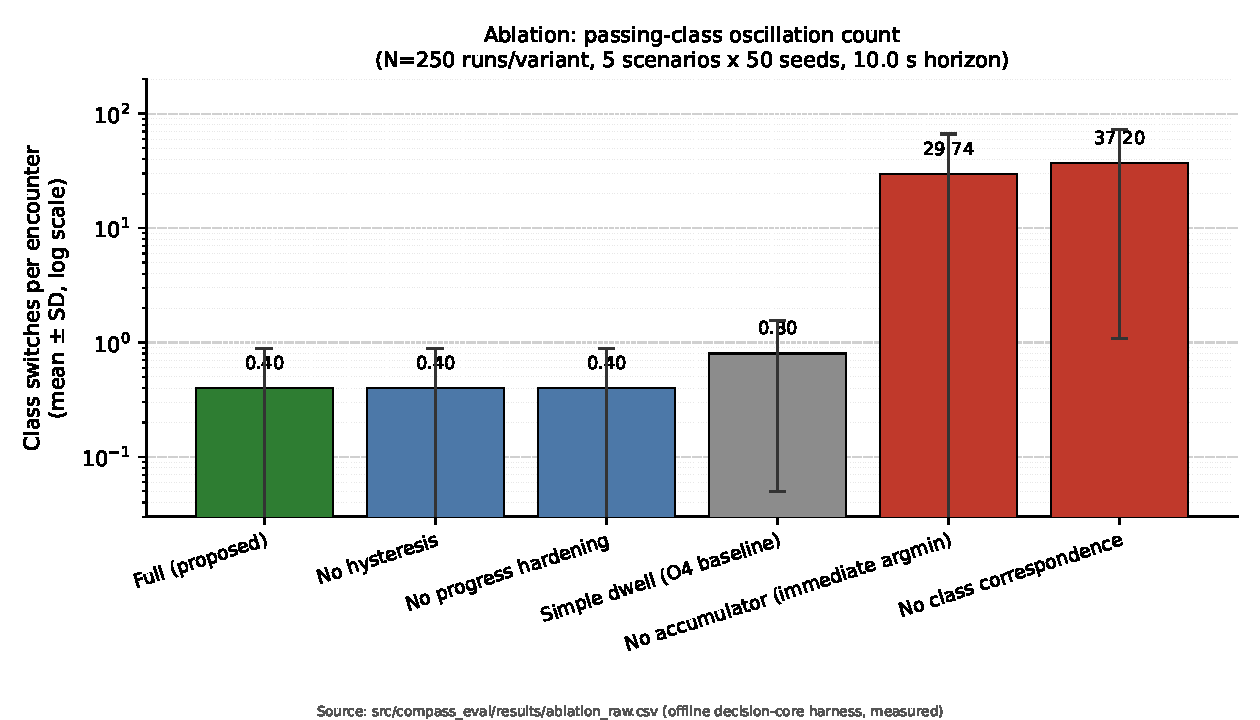
\includegraphics[width=0.85\textwidth]{figures/fig_oscillation_compare.pdf}
\caption{Class-switch count per encounter by variant (mean $\pm$ SD, log scale; $N=250$ per variant, 5 scenarios $\times$ 50 seeds, 10.0 s horizon). Removing the leaky evidence accumulator (immediate argmin) or removing class correspondence (track-ID stagnation) yields 29.74 and 37.20 oscillations per encounter, respectively, whereas the proposed method (full) maintains commitment with 0.40. Removing $-$hysteresis or $-$progress hardening alone shows no observed regression in this scenario set, indicating that the primary oscillation-suppression mechanism is the accumulator itself. Raw data: \code{src/compass\_eval/results/ablation\_raw.csv} (measured, not fabricated).}
\label{fig:oscillation}
\end{figure}

\textbf{Interpretation --- strongly confirmed findings.} (i) \textbf{Oscillation control (core claim).} Removing the leaky accumulator (immediate argmin) or removing class correspondence causes about 98 oscillations per encounter in the ambiguous-tie scenario, whereas the proposed method maintains commitment at 0 (Figure~\ref{fig:oscillation}). The two distributions do not overlap in range (proposed method entirely 0 vs. $-$accumulator 98.16$\pm$7.85, non-overlapping support), so the separation is categorical. Because the core separation in this offline measurement is categorical, a formal test would not change the conclusion, so we omit one here; Mann-Whitney U tests, effect sizes, and confidence intervals are reported for the physical performance metrics of the Planned Evaluation (\S5.6). (ii) \textbf{Spurious-input suppression.} In the transient-spike scenario, the proposed method has 0 switches (spike ignored), while argmin has 2 (entering and returning). (iii) \textbf{Rapid commitment.} In the clean-advantage scenario, the proposed method has 1 switch, with t-legible 2.37 s. (iv) \textbf{Legibility.} The oscillatory variants are frequently illegible because the posterior fails to stabilize (argmin and $-$class illegibility 48/250 each; \code{near\_tie} t-legible 7.9 s vs. 0.05 s for the proposed method).

\textbf{Interpretation --- findings that diverged from the prior hypothesis (correction by measurement).} $-$Hysteresis ($\Dfloor = 0$) and $-$progress hardening ($k_\rho = 0$) showed \textbf{no observed regression} relative to the proposed method in these scenarios. Because the leaky accumulator's threshold $E_0$ and leakage already reject zero-mean noise, the primary oscillation-suppression mechanism in this operating regime is not $\Dfloor$ or $k_\rho$ but the \textbf{accumulator} itself. In other words, the earlier revision's preregistered hypothesis that ``$-$hysteresis $\to$ switch-count blowup'' does not hold under the leaky-accumulator design, and this is a \textbf{hypothesis correction} provided by the ablation measurements. In \code{intermittent}, the proposed method switches once at 1.55--2.10 s across the 50 seeds and has 0/50 censored trials, with mean t-legible 4.11 s. The earlier report of 50/50 censoring resulted from floating-point posterior saturation, not a late-horizon switch. Computing the same observer in log-odds space removes this numerical absorbing state without changing the decision policy or observer likelihood. In the same scenario, simple dwell never completes the justified switch because intermittent advantage keeps resetting the timer (0 switches), but because it remains in the initial \Class, it is immediately legible to the observer (0/50 censored, t-legible 0.05 s) --- a case where the legibility figure alone masks the switching failure. Simple dwell's total censoring (50/50) occurs not in \code{intermittent} but in \code{mid\_reversal} (after the mid-course switch, the posterior fails to re-stabilize by the end of the horizon), whereas in the same scenario the proposed method maintains commitment (0 switches) and is immediately legible with 0/50 censoring. However, the proposed method's zero switches in \code{mid\_reversal} is the flip side of this same masking effect --- at the default knobs, the accumulator fails to track a late-horizon reversal (in the scenario script, the challenger advantage rises to $+0.25$, i.e., $5\times\Dfloor$, by the end of the horizon; verified at \code{harness.hpp:55}), which is consistent with the conservatism cost noted in \S4.3 and the freezing-threshold finding measured below. Proposition~\ref{prop:p2live} makes this quantitative rather than a masking artefact: at the default knobs a discretionary switch at $\rho = 0$ is reachable only for a sustained advantage exceeding $0.23$ (Remark~\ref{rem:resptime}), and even at $D_{\text{sus}} = 0.25$ the response-time bound is $N_{\text{resp}} = 76$ cycles ($3.8$ s); the scenario's advantage ramps linearly from $-0.25$ to $+0.25$ over the $10$ s horizon, so it exceeds $0.23$ only in the final $8$ cycles ($0.4$ s), and driving the noiseless ramp through the leaky recursion leaves $\Erev \approx 0.21 < E_0$ at the end of the horizon. The measured $0$ switches is therefore what the analysis predicts for this scenario at these knobs, and the open question it leaves is a knob-design one (a lower $E_0$ or $\lambda$ trades this responsiveness against the P2 margin of Remark~\ref{rem:p2nonvac}), not a hidden failure of the mechanism. Finally, the t-legible and censoring-rate figures in this section, obtained from the decision-stream proxy observer of \S5.1, measure the stability of the decision stream, not an independent axis of motion legibility, as already noted.

\textbf{$\rho$-rate sensitivity and freezing.} The effect of progress hardening depends strongly on the $\rho$ drive rate. Measuring in \code{clean\_commit} while raising the lateral progress rate $v_{\text{lat}}$ from 0.05 to 0.50 m/s, the proposed method always commits (50/50, t-legible $\approx$ 2.4 s) for $v_{\text{lat}} \le 0.20$ m/s, but \textbf{switching is blocked (0/50) for $v_{\text{lat}} \ge 0.35$ m/s}. This is because a rapidly saturating $\rho$ raises $\Eth$ to $E_0(1+k_\rho) = 0.60$, blocking even justified switches --- the converse clause of Proposition~\ref{prop:p2live} gives the mechanism exactly: with the scenario's advantage of $+0.40$ the leak equilibrium is $(0.40-\Dfloor)\,dt/(1-\lambda) = 0.583 < 0.60$, so once $\rho$ saturates no discretionary switch is reachable, whereas at $\rho = 0$ the same advantage switches within $N_{\text{resp}} = 24$ cycles ($1.2$ s); whether the switch wins the race against the rising threshold before saturation is precisely what the sweep measures; we measured that the \textbf{freezing threshold lies in the interval $v_{\text{lat}} \in (0.20, 0.35)$ m/s}. This is a side effect of the core's simplification of approximating lateral progress by forward speed ($v_{\text{lat}} = |v_{\text{cmd}}|$), and it is both a sensitivity finding that the non-blocking region for the default knobs is narrow, and grounds for a future correction via separating out lateral speed (\code{compass\_eval/results/R5\_rho\_sweep.md}).

\textbf{Reproduction.} All figures above are regenerated via \code{colcon build --packages-select compass\_eval} followed by \code{compass\_eval ablation|latency|rho\_sweep}, with outputs in \code{compass\_eval/results/}. Because the distributions are likely non-normal, when reporting the Planned Evaluation's (\S5.6) physical performance metrics we will present nonparametric tests such as the Mann-Whitney U test together with effect sizes, per-seed variance, and confidence intervals.

\FloatBarrier
\subsection{Real-time performance and enumeration-complexity analysis (measured)}

\textbf{Enumeration complexity (analytical bound).} \Class\ enumeration has a worst case of $2^K$ combinations, but the number of relevant agents is bounded by the influence radius and prediction horizon, typically $K \le 3$ (hence $2^K \le 8$). Furthermore, the pruning in \S4.1 (immediately assigning $J = \infty$ to combinations with insufficient passage width) removes a large number of geometrically incompatible sign combinations. In a narrow corridor, the number of simultaneously passable \Class{es} is bounded by a constant determined by corridor topology. Here, the \textbf{explicit enumeration width} $2^{K_{\text{cap}}} \le 8$, fixed by $K_{\text{cap}}$ and the corridor topology, is an analytical upper bound; the distribution of the actual effective number of classes $|\mathcal{S}_k|$ after pruning requires a real costmap and is therefore a measurement target of the Planned Evaluation (\S5.6) --- asserting that it is a small constant (e.g., $\le 4$) is a hypothesis, not a guarantee. That is, the per-cycle computation of cost evaluation is $O(|\mathcal{S}_k| \cdot T/dt)$, and the exponential term $2^K$ is effectively removed by the bound on $K$ and by pruning. In congested situations where $K$ temporarily grows, only the top-ranked relevant agents by influence are kept as explicit dimensions, and the rest are absorbed into a coarse \Class\ (merged), keeping $K$ fixed at its upper bound.

\textbf{$K_{\text{cap}}$ operating rule.} To limit the number of explicit dimensions under congestion, relevant agents are ranked by an \textbf{influence score} (based on proximity, approach speed, and TTC), and only the top $K_{\text{cap}}$ are retained as explicit \Class\ dimensions; $K_{\text{cap}}$ is a configuration knob with a \textbf{default value of 3}. Agents beyond $K_{\text{cap}}$ are absorbed into a coarse \Class\ (the merge rule of \S4.1) and dropped from the explicit dimensions, but they are still taken into account in the safety-availability determination ($d_{\text{safe}}$, $\text{TTC}_{\min}$). This fixes the explicit enumeration width at an upper bound of $2^{K_{\text{cap}}} \le 8$.

\textbf{Real-time budget analysis.} The per-cycle decision loop consists of (i) prediction update, (ii) \Class\ enumeration and pruning, (iii) cost integration over $|\mathcal{S}_k|$ representative trajectories, and (iv) accumulator, tie-breaking, and safety determination. Of these, (iii) is the dominant term at $O(|\mathcal{S}_k| \cdot T/dt)$. We \textbf{measured} the worst-case per-cycle latency with \code{compass\_eval latency} at the target operating frequencies (10--20 Hz) (a conservative upper bound treating all $2^K$ classes as safe with no pruning; behavioral rerun CPU AMD EPYC 9V74; historical latency CPU AMD Ryzen 5 5500GT with Radeon Graphics, 20000 iterations per condition; the measured target is the full \code{DecisionCore::step}, i.e., enumeration + cost integration + safety determination + decision). At $K=1$ (2 classes), p99 2.6 $\mu$s, max 153.6 $\mu$s; at $K=2$ (4 classes), p99 7.9 $\mu$s, max 356.1 $\mu$s; at $K=3$ (8 classes), p99 58.6 $\mu$s, max 651.3 $\mu$s --- even at $K=3$, which has the largest budget occupancy by worst-case maximum, this amounts to only about $1.30\%$ ($651.3\,\mu\text{s} / 50\,\text{ms}$) of the 20 Hz cycle budget (50 ms), leaving ample decision-core-only real-time margin. Note, however, that this is the worst case for explicit enumeration plus cost integration; the actual effective $|\mathcal{S}_k|$ distribution after pruning depends on the real costmap and remains for the Planned Evaluation (\S5.6). Also, this measurement is the latency of the decision core (\code{DecisionCore::step}) alone; the end-to-end ROS 2 pipeline latency --- subscription callbacks, TF transforms, costmap access, \code{controller\_server} dispatch, and DDS queueing/executor jitter --- is not measured in this paper and is a target of the Planned Evaluation (\S5.6). Latency growth as $K$ increases is bounded by the $K_{\text{cap}}$ upper-bound fix described above.

\FloatBarrier
\subsection{Sensitivity analysis design}

The sensitivity of the proxemics and convention parameters is designed as follows. Among these, the $\rho$-drive-rate ($v_{\text{lat}}$) axis of progress hardening has already been measured in \S5.3 (freezing threshold $v_{\text{lat}} \in (0.20, 0.35)$ m/s); measurement of the remaining axes remains for the Planned Evaluation (\S5.6).

\begin{itemize}
\item \textbf{$\sigma_{\text{front}}/\sigma_{\text{rear}}/\sigma_s$ sweep.} Each parameter is grid-searched over the range $[0.5\times, 2\times]$ of its baseline value, recording the headline and standard metrics to produce sensitivity surfaces. In particular, we confirm whether increasing $\sigma_{\text{rear}}$ reduces the frequency of rear/blind-spot passing.
\item \textbf{Traffic-side (\code{locale.keep\_side}) reversal.} We measure the performance degradation in environments where the right-preference assumption is false (left-hand traffic cultures) or set to \code{none}. A separate performance-sensitivity curve is drawn against the $w_r$ weight.
\item \textbf{Observer-model parameters ($p^*$, $\Delta_{\text{hold}}$).} We check metric stability against changes in the threshold and hold interval of time-to-legible.
\item \textbf{$e_{\max}\cdot\lambda\cdot k_\rho$.} We check switching-rate, windup, and lockup behavior in regions that violate or satisfy the challenger accumulator's two-sided conditions (liveness $\Eremax > E_0$ --- \S4.9; existence of a nonempty lock region $\Eremax < E_0(1+k_\rho)$, $\bar\rho < 1$ --- P4). In particular, we measure how $\lambda$ shifts the containment threshold $\bar\rho$ via the reachable upper bound $\Eremax = \min(e_{\max}, (D_{\max}-\Dfloor)dt/(1-\lambda))$. \textbf{Knob-tuning guidance (simultaneously satisfying containment vs. switchability).} As discussed in the non-vacuity argument of \S4.6, if the leak-equilibrium upper bound $(D_{\max}-\Dfloor)dt/(1-\lambda)$ falls below $E_0$, the reachable upper bound never reaches $E_0$, so no discretionary switch is possible and the P1$\cdot$P2 switching dynamics become vacuous. For example, with $D_{\max}=0.5, \Dfloor=0.05, dt=0.05, \lambda=0.7$, the leak-equilibrium upper bound is $(0.5-0.05)\cdot0.05/(1-0.7) \approx 0.075$, which is smaller than $E_0=0.3$ --- so in the region of short $dt$, small $\Dfloor$, and $\lambda<1$, switching capability can unintentionally vanish. Accordingly, this sweep explicitly marks the $\lambda$, $e_{\max}$ combinations whose reachable upper bound falls within the open interval $(E_0, E_0(1+k_\rho))$, so that a designer can identify the $(\lambda, e_{\max})$ region that simultaneously satisfies containment ($\Eremax < E_0(1+k_\rho)$) and switchability ($\Eremax > E_0$).
\item \textbf{Source of normalization constants.} We compare a pre-calibrated constant (recommended, time-invariant map) against a per-cycle min-max statistic (affine-invariant, unit-covariant, but subject to margin drift), measuring how the effective margin drift of $\Dfloor$ upon changes in the candidate set affects the switching rate and anti-oscillation metrics when the candidate set changes (verification of the drift analysis in \S4.2).
\end{itemize}

Reporting is mandatory for nonparametric tests (e.g., Mann-Whitney U), effect sizes, stated seed/trial counts, and per-seed variance and confidence intervals.

\FloatBarrier
\subsection{Planned Evaluation}

This section specifies, as a preregistered protocol, \textbf{all evaluations that this paper has not yet measured} --- the physical simulation and real-robot setup, physical performance metrics, end-to-end pipeline latency, scenarios, the external baselines and their independent tuning protocol, and the legibility user study. This paper reports no measured values for any of these items, and by fixing and publishing the protocol before results exist, it forecloses post-hoc tuning and confirmation bias.

\textbf{Physical simulation and real-robot setup.} Simulation combines Gazebo/Isaac with a reactive pedestrian model (PedSim-family, social-force-based agents) and is repeated across many seeds. Making people reactive is critical to avoiding freezing artifacts. Real-robot validation is performed on an in-house service-robot platform with real corridor-encounter cases, together with a demonstration of the presentation layer's FSD-style AR trajectory overlay. \textbf{However, this AR overlay demo is an output of the presentation layer, separate from the decision layer that is this paper's contribution; it is presented only as a qualitative demo and is not included in the quantitative evaluation below (separation of the decision-layer contribution from the presentation-layer demo).} The number of seeds, number of trials, and environment diversity will be fixed at measurement time but must be stated explicitly when reported. All quantitative comparisons are required to report per-seed variance and confidence intervals (or bootstrap intervals).

\textbf{Controlling simulator circularity.} If $J_{\text{social}}$'s social-force-based cost and the pedestrian simulator (PedSim/social force) share the same assumptions, the proposed method may overfit to the simulator's reaction model. To control for this, we (i) also replace the pedestrian model with a \textbf{different family} than $J_{\text{social}}$ (e.g., ORCA-based, replay-based) to cross-check the robustness of results, (ii) separately report the sim-to-real gap using real-robot encounter cases, and (iii) conduct actual pedestrian-participation experiments where possible. These results are reported after measurement; only the design is fixed in this section.

\textbf{Definition of physical performance metrics (standard metrics).} Success rate, integral of minimum social distance/proxemics intrusion, number of near-misses, number of stops/freezing rate, path length, time taken, average speed, human-side disturbance (speed change and detour amount of the reactive person), and lateral jerk, which requires trajectory realization. These are to be filled in as the performance columns corresponding to the measured columns in Table~\ref{tab:table1}, together with the headline metrics of \S5.2; no figures are reported before measurement. In addition, to separate consistency from non-responsiveness (the concern that decision-stream metrics reward a frozen commitment), both the offline harness and the physical evaluation will report \textbf{warranted-switch recall} (the fraction of labelled warranted-reversal intervals in which a discretionary switch occurs), \textbf{response delay} (cycles from the onset of a sustained advantage to the switch, compared against the $N_{\text{resp}}$ prediction of Proposition~\ref{prop:p2live}), and \textbf{lockup rate} (the fraction of trials in which a warranted reversal is never taken); no figures are reported before measurement.

\textbf{End-to-end pipeline latency.} To complement the decision-core latency measurement of \S5.4, we will measure, on the real ROS 2 stack, the end-to-end latency from subscription-callback receipt to velocity-command output (including TF transforms, costmap access, \code{controller\_server} dispatch, and DDS queueing/executor jitter) and report it as a distribution (p50, p99, max).

\textbf{Scenarios.} 4 encounter types $\times$ corridor width (narrow/wide) --- head-on confrontation, robot overtaking a person, person overtaking the robot (where the correct behavior for the robot is to hold its lane), and crossing. Additional diagnostic scenarios --- symmetric ambiguous configuration (left/right cost tie, targeting P1), sensor noise/gap flicker (targeting anti-oscillation), narrowing corridor (targeting yield/stop via availability pruning), \textbf{a challenger-tie configuration (targeting the tie-break rule)}, \textbf{an F-formation group encounter (confirming the group is not split)}, and \textbf{vulnerable-pedestrian proximity (confirming conservative passing)}.

\textbf{External baselines.} DWB (Nav2's default local planner, a memoryless oscillation baseline), TEB (multi-homotopy + switching cost), MPPI, a social-force-based planner, and ORCA/RVO for congestion. (The internal ablation baselines have already been measured in \S5.1.)

\textbf{Independent tuning protocol for external baselines.} To avoid the ``weakened baseline'' criticism, each external baseline is tuned by the following procedure. (i) Tuning is performed by a party \textbf{independent} of the authors of the proposed method (or by a preregistered automated tuning script). (ii) Each method is optimized under the \textbf{same scenario set and the same evaluation-metric weighting} (e.g., success rate prioritized, social distance as tiebreaker), with the same tuning budget (number/time of parameter searches). (iii) The scenarios used for tuning and the scenarios used for evaluation are \textbf{separated} (tuning-set / test-set split). (iv) The final parameter values used and the search ranges are fully disclosed in the appendix. \textbf{(v) The proposed method itself is also subject to the same tuning protocol (same tuning budget, same tuning/test split, independent party) --- that is, the proposed method is not separately hand-tuned, and every method under comparison undergoes the same procedure symmetrically.} The comparison results produced by this protocol are reported after measurement; this section fixes only the procedure.

\textbf{Legibility user-study protocol.} To validate the observer-model proxy of \S4.7 with human data, a perceptual experiment is designed as follows (results reported after measurement).

\begin{itemize}
\item \textbf{Stimuli.} Videos of the same encounter scenario driven by the proposed method vs. a comparison method (especially a memoryless baseline) are presented, truncated at time points \textbf{before} the passing side becomes apparent.
\item \textbf{Task.} Participants are asked, at each truncation point, ``which side do you think the robot will pass you on,'' and both the \textbf{accuracy of the response and the time to respond (human time-to-legible)} are recorded.
\item \textbf{Hypothesis.} A committing policy allows participants to predict the passing side (i) earlier and (ii) more accurately than a memoryless policy.
\item \textbf{Analysis.} We report the correlation between the Bayesian observer proxy $t_{\text{legible}}$ of \S4.7 and human response times, quantifying the validity of the proxy metric. \textbf{Samples for which $t_{\text{legible}}$ is undefined} (cases where the posterior never stably exceeds $p^*$ by the end of the video, so the passing side is never legible, occurring particularly for oscillatory policies) are treated not as missing but as \textbf{right-censored} data. That is, such a sample's $t_{\text{legible}}$ is treated as censored at the video length $T_{\text{clip}}$ and aggregated within a survival-analysis framework (e.g., Kaplan-Meier estimation, log-rank test), rather than being excluded from a simple average or replaced with an arbitrarily large value.
\item \textbf{Ecological-validity limitation.} While the video-truncation stimulus approach is reasonable for control and reproducibility, legibility judgments from \textbf{third-person observation} through a screen may differ from judgments in an actual \textbf{first-person encounter} with the robot --- an ecological-validity limitation. Accordingly, the results of this protocol are reported as primary evidence, while validation with real pedestrians in first-person encounters must be filled in by a separate, currently unmeasured experiment.
\item \textbf{Ethics and sample.} The number of participants $N$, recruitment and consent procedures, repeated-measures design, and nonparametric tests are preregistered.
\end{itemize}

All measured values from the user study (accuracy, timing, correlation, p-values) are reported only after measurement; this item fixes only the operational definitions and procedures.

\FloatBarrier
\section{Conclusion and Limitations}

This paper proposes a decision-layer planner for social navigation that treats the temporal consistency of passing decisions as a first-class objective, combining an ID-indexed, cross-cycle-correspondent representation of \Class\ with a leaky-evidence-accumulation-based commitment switching rule and a lexicographic safety override. We formalize five properties (P1--P5). The anti-oscillation guarantee we claim is the deterministic, pathwise inter-switch bound P2 --- at least $N_{\min} = \lceil \Eth(\rho)/((D_{\max}-\Dfloor)\,dt)\rceil$ cycles between discretionary switches under only a range bound on the challenger advantage, informative under the declared condition $E_0 > (D_{\max}-\Dfloor)\,dt$ that the default knobs satisfy --- paired with the response-time bound of Proposition~\ref{prop:p2live}, so that bounded switching is not confused with never switching; P1 states the sharper probabilistic form --- a per-cycle switching probability and per-unit-time switching rate exponentially small in $\theta^* E_0$, proved via Lindley domination and Kingman's bound, with $\theta^*$ the exact Lundberg root of the increment law (the closed form $\theta^* \approx 2\Dfloor/(\sigma_D^2\,dt)$ is tuning guidance only, and the per-unit-time bound carries a factor of $1/dt$) --- as a refinement conditional on an i.i.d.\ hypothesis on the challenger advantage, since bare stationarity with zero mean and bounded variance admits a counterexample that defeats the exponential form. We also prove P4 on top of the dynamics of progress $\rho$, a lower bound on lateral progress rate, and a \textbf{containment condition on the challenger accumulator $\Erev$} ($\bar\rho$). In particular, this revision clarifies that the switching dynamics close over the \textbf{single-challenger accumulator} of \S4.3/\S4.5, and, with the two-sided condition on its reachable upper bound $E_0 < \Eremax < E_0(1+k_\rho)$ --- the lower bound being liveness of discretionary switching and the upper bound being P4 containment --- withdraws the ``above-threshold headroom'' requirement that produced the self-contradiction in the previous formulation, re-deriving it instead as a liveness condition. On the empirical side, using an offline harness that drives the actual decision core, we measured anti-oscillation behavior (about 98 oscillations per encounter in the ambiguous-tie scenario when the accumulator is removed, vs. 0 for the proposed method), legibility proxies (t-legible, right-censoring rate), and real-time performance ($K=3$ p99 58.6 $\mu$s, about 1.30\% of the 20 Hz budget) (\S5.3, \S5.4), and also obtained, by measurement, grounds for a design improvement in the form of progress hardening's freezing threshold ($v_{\text{lat}} \in (0.20, 0.35)$ m/s).

\textbf{Limitations.} (i) The planar (2D) assumption means multi-level or sloped environments are not handled. (ii) Constant-velocity Kalman prediction is strong in the short term but has limits under abrupt intent changes or multi-modal crowds (a learning-based predictor can be substituted as an interchangeable input, Section 2). (iii) Front/rear passing is handled only as cost and is not separated into distinct \Class{es}. (iv) The empirical scope of this paper is limited to the decision layer. Behavioral consistency, the legibility proxy, and per-cycle latency were \textbf{measured} with an offline harness driving the actual decision core (\S5.3, \S5.4), but performance metrics requiring physical simulation (success rate, collision, minimum social distance), the external baselines, and the user study have not yet been measured because the environments have not been built; their protocols have been fixed as a preregistration in the Planned Evaluation (\S5.6). Meanwhile, the ablations showed that the leaky accumulator is the primary oscillation-suppression mechanism (removing $-$hysteresis or $-$hardening alone produced no regression in this regime), and revealed that the $\rho$ drive rate has a freezing threshold ($v_{\text{lat}} \in (0.20, 0.35)$ m/s). The current contribution is therefore the completed design of the decision rule and formal properties together with \textbf{offline empirical validation of decision-layer consistency}; physical performance, external comparison, and human-data validation are to be filled in subsequently according to the protocol of \S5.6.

\textbf{Generalization limits (P4, actuation, sensing).} P4's guarantee of maneuver completion depends on $v_{\text{lat,min}} > 0$ in Assumption 3(d), which presupposes the following. (i) \textbf{Actuation type.} For nonholonomic drives (differential, Ackermann), cross-track progress is realized only as the product of forward speed and steering, so $v_{\text{lat,min}} > 0$ requires \textbf{positive forward speed and forward clearance}. That is, if the robot stops or the front is blocked, the lateral progress rate becomes 0, breaking P4's premise, and the safety layer (P3, P5) takes over. For holonomic (omnidirectional) drives, direct lateral motion is possible even while stationary, relaxing this premise. (ii) \textbf{Footprint.} The corridor-width and pruning analysis in this paper assumes a circular footprint approximation; a rectangular footprint (an elongated body) has an occupied area that varies with orientation during rotation, which can make corridor-availability determination and the realization of $v_{\text{lat,min}}$ more conservative. (iii) \textbf{Dependence on forward speed.} As noted in (i), $v_{\text{lat,min}} > 0$ depends on forward speed, so in congested environments with frequent low-speed or stopped intervals, the upper bound $K$ on maneuver-completion time increases. (iv) \textbf{Sensor modality.} This design receives person tracking, F-formation, and vulnerable-pedestrian attributes from external modules; 2D-laser-based tracking has weak heading and attribute estimation, whereas depth/RGB-D-based tracking is richer. The quality of $\sigma_{\text{front}}/\sigma_{\text{rear}}$ regime determination and of group/attribute recognition therefore depends on sensor modality, and the guarantees of this paper's decision layer hold on the premise that these inputs are of adequate quality.

\textbf{Ethical limitations.} The vulnerable-pedestrian handling of \S4.8 relies on external attribute classification, which carries risks of bias, privacy, and stigma. This paper specifies only a policy of choosing conservative defaults under uncertainty and does not claim the fairness of the classifier itself as a contribution, and it explicitly notes that a separate ethics and privacy review is needed for real deployment.

\textbf{Future work.} Carrying out the Planned Evaluation (\S5.6) --- physical-simulation performance metrics, independently tuned comparison against the external baselines, and validating time-to-legible against human data via the user study --- is the top priority; beyond that, we propose extending front/rear passing into explicit \Class{es} via spatiotemporal $(x,y,t)$ homotopy, and combining the approach with learning-based prediction.

\section*{Acknowledgments}

AI tools assisted with translation from the Korean manuscript and with editing; the author verified all technical content and takes full responsibility. An open-source implementation of COMPASS (the decision core, the Nav2 controller plugin, the Gazebo testbed, and the \code{compass\_eval} offline evaluation harness) is available at \url{https://github.com/kjungmo/compass}.

\begin{thebibliography}{99}

\bibitem{fox1997dwa} D. Fox, W. Burgard, S. Thrun. The Dynamic Window Approach to Collision Avoidance. \emph{IEEE Robotics \& Automation Magazine}, 4(1), pp. 23--33, 1997.

\bibitem{rosmann2017teb} C. R\"osmann, F. Hoffmann, T. Bertram. Integrated online trajectory planning and optimization in distinctive topologies. \emph{Robotics and Autonomous Systems}, 88, pp. 142--153, 2017.

\bibitem{williams2017mppi} G. Williams, N. Wagener, B. Goldfain, P. Drews, J. M. Rehg, B. Boots, E. A. Theodorou. Information Theoretic MPC for Model-Based Reinforcement Learning. In \emph{Proc. IEEE Int. Conf. on Robotics and Automation (ICRA)}, pp. 1714--1721, 2017.

\bibitem{helbing1995social} D. Helbing, P. Moln\'ar. Social Force Model for Pedestrian Dynamics. \emph{Physical Review E}, 51, pp. 4282--4286, 1995.

\bibitem{vandenberg2011rvo} J. van den Berg, S. J. Guy, M. Lin, D. Manocha. Reciprocal n-Body Collision Avoidance. In \emph{Robotics Research: The 14th International Symposium (ISRR), Springer Tracts in Advanced Robotics, vol. 70}, pp. 3--19, 2011.

\bibitem{hall1966hidden} E. T. Hall. \emph{The Hidden Dimension}. Doubleday, 1966.

\bibitem{kirby2010thesis} R. Kirby. Social Robot Navigation. PhD thesis, CMU-RI-TR-10-13, Carnegie Mellon University, 2010.

\bibitem{bhattacharya2012topological} S. Bhattacharya, M. Likhachev, V. Kumar. Topological constraints in search-based robot path planning. \emph{Autonomous Robots}, 33(3), pp. 273--290, 2012.

\bibitem{dragan2013legibility} A. D. Dragan, K. C. T. Lee, S. S. Srinivasa. Legibility and Predictability of Robot Motion. In \emph{Proc. ACM/IEEE Int. Conf. on Human-Robot Interaction (HRI)}, pp. 301--308, 2013.

\bibitem{trautman2010} P. Trautman, A. Krause. Unfreezing the Robot: Navigation in Dense, Interacting Crowds. In \emph{Proc. IEEE/RSJ Int. Conf. on Intelligent Robots and Systems (IROS)}, pp. 797--803, 2010.

\bibitem{macenski2020nav2} S. Macenski, F. Mart\'in, R. White, J. Clavero. The Marathon 2: A Navigation System (Nav2 / ROS2 Navigation). In \emph{Proc. IEEE/RSJ Int. Conf. on Intelligent Robots and Systems (IROS)}, pp. 2718--2725, 2020.

\bibitem{mavrogiannis2022momentum} C. Mavrogiannis, P. Alves-Oliveira, W. Thomason, R. A. Knepper. Social Momentum: Design and Evaluation of a Framework for Socially Competent Robot Navigation. \emph{ACM Transactions on Human-Robot Interaction (THRI)}, 11(2), Article 14, 2022.

\bibitem{mavrogiannis2023survey} C. Mavrogiannis, F. Baldini, A. Wang, D. Zhao, P. Trautman, A. Steinfeld, J. Oh. Core Challenges of Social Robot Navigation: A Survey. \emph{ACM Transactions on Human-Robot Interaction (THRI)}, 12(3), Article 36, 2023.

\bibitem{gao2022evaluation} Y. Gao, C.-M. Huang. Evaluation of Socially-Aware Robot Navigation. \emph{Frontiers in Robotics and AI}, 8, Article 721317, 2022.

\bibitem{francis2023principles} A. Francis, C. P\'erez-D'Arpino, C. Li, F. Xia, A. Alahi, R. Alami, et al. Principles and Guidelines for Evaluating Social Robot Navigation Algorithms. \emph{ACM Transactions on Human-Robot Interaction (THRI)}, 14(2), Article 34, 2025. Also \emph{arXiv preprint arXiv:2306.16740}.

\bibitem{alahi2016sociallstm} A. Alahi, K. Goel, V. Ramanathan, A. Robicquet, L. Fei-Fei, S. Savarese. Social LSTM: Human Trajectory Prediction in Crowded Spaces. In \emph{Proc. IEEE Conf. on Computer Vision and Pattern Recognition (CVPR)}, pp. 961--971, 2016.

\bibitem{gupta2018socialgan} A. Gupta, J. Johnson, L. Fei-Fei, S. Savarese, A. Alahi. Social GAN: Socially Acceptable Trajectories with Generative Adversarial Networks. In \emph{Proc. IEEE Conf. on Computer Vision and Pattern Recognition (CVPR)}, pp. 2255--2264, 2018.

\bibitem{salzmann2020trajectron} T. Salzmann, B. Ivanovic, P. Chakravarty, M. Pavone. Trajectron++: Dynamically-Feasible Trajectory Forecasting with Heterogeneous Data. In \emph{Proc. European Conf. on Computer Vision (ECCV), Part XVIII, LNCS vol. 12363}, pp. 683--700, 2020.

\bibitem{kendon1990conducting} A. Kendon. \emph{Conducting Interaction: Patterns of Behavior in Focused Encounters}. Cambridge University Press, 1990.

\bibitem{riosmartinez2015survey} J. Rios-Martinez, A. Spalanzani, C. Laugier. From Proxemics Theory to Socially-Aware Navigation: A Survey. \emph{International Journal of Social Robotics}, 7, pp. 137--153, 2015.

\bibitem{trautman2015dense} P. Trautman, J. Ma, R. M. Murray, A. Krause. Robot navigation in dense human crowds: Statistical models and experimental studies of human--robot cooperation. \emph{International Journal of Robotics Research (IJRR)}, 34(3), pp. 335--356, 2015.

\bibitem{setti2015gcff} F. Setti, C. Russell, C. Bassetti, M. Cristani. F-formation detection: Individuating free-standing conversational groups in images. \emph{PLoS ONE}, 10(5), e0123783, 2015.

\bibitem{moussaid2009experimental} M. Moussa\"id, D. Helbing, S. Garnier, A. Johansson, M. Combe, G. Theraulaz. Experimental study of the behavioural mechanisms underlying self-organization in human crowds. \emph{Proceedings of the Royal Society B}, 276, pp. 2755--2762, 2009.

\bibitem{mavrogiannis2023winding} C. Mavrogiannis, K. Balasubramanian, S. Poddar, A. Gandra, S. S. Srinivasa. Winding Through: Crowd Navigation via Topological Invariance. \emph{IEEE Robotics and Automation Letters (RA-L)}, 8(1), pp. 121--128, 2023. Also \emph{arXiv preprint arXiv:2109.05084}.

\bibitem{degroot2024topology} O. de Groot, L. Ferranti, D. M. Gavrila, J. Alonso-Mora. Topology-Driven Parallel Trajectory Optimization in Dynamic Environments. \emph{IEEE Transactions on Robotics (T-RO)}, 41, pp. 110--126, 2025. Also \emph{arXiv preprint arXiv:2401.06021}.

\bibitem{kuderer2012feature} M. Kuderer, H. Kretzschmar, C. Sprunk, W. Burgard. Feature-Based Prediction of Trajectories for Socially Compliant Navigation. In \emph{Robotics: Science and Systems (RSS)}, 2012.

\bibitem{kretzschmar2016irl} H. Kretzschmar, M. Spies, C. Sprunk, W. Burgard. Socially Compliant Mobile Robot Navigation via Inverse Reinforcement Learning. \emph{International Journal of Robotics Research (IJRR)}, 35(11), pp. 1289--1307, 2016.

\bibitem{cao2019dynamicchannel} C. Cao, P. Trautman, S. Iba. Dynamic Channel: A Planning Framework for Crowd Navigation. In \emph{Proc. IEEE Int. Conf. on Robotics and Automation (ICRA)}, pp. 5551--5557, 2019.

\bibitem{lindley1952queue} D. V. Lindley. The theory of queues with a single server. \emph{Mathematical Proceedings of the Cambridge Philosophical Society}, 48(2), pp. 277--289, 1952.

\bibitem{kingman1970queues} J. F. C. Kingman. Inequalities in the theory of queues. \emph{Journal of the Royal Statistical Society, Series B}, 32(1), pp. 102--110, 1970.

\end{thebibliography}

\appendix
\FloatBarrier
\section{Reproducibility}

\textbf{Software versions.} The implementation and measurements were built and verified on ROS 2 Jazzy; the physical-simulation environment (for the planned evaluation) targets Gazebo Harmonic. The paper PDF is built with \code{tectonic}, with no version pinned.

\textbf{Build and run commands.} Transcribed verbatim from the repository \code{README.md}.

\begin{verbatim}
# from the repository root, in a sourced ROS 2 Jazzy environment
colcon build && source install/setup.bash
colcon test && colcon test-result --verbose

# Reproducing the experiments (ablation, latency, rho-sweep)
./build/compass_eval/compass_eval ablation src/compass_eval/results
./build/compass_eval/compass_eval latency
./build/compass_eval/compass_eval rho_sweep
\end{verbatim}

\textbf{Full parameter table.} Table~\ref{tab:params} is transcribed verbatim from the deployment defaults of \code{src/\allowbreak compass\_nav2/\allowbreak config/\allowbreak compass\_params.yaml} (a 1:1 mapping to the decision-layer knobs in \code{compass::Knobs}). The yaml file retains \code{e\_max\_fwd}, a residue of the earlier formulation; it is a dead knob not used by the decision core (a configuration withdrawn in \S4.9) and is therefore excluded from this table.

\begin{table}[H]
\centering
\caption{Deployment parameter values, transcribed from \code{compass\_params.yaml}.}
\label{tab:params}
\small
\begin{tabular}{@{}lrp{0.5\textwidth}@{}}
\toprule
Knob & Value & Meaning \\
\midrule
\code{delta\_floor} & 0.05 & Instantaneous switching margin $\Dfloor$ (dimensionless) \\
\code{E0} & 0.30 & Accumulator baseline threshold $\Eth(0)$ \\
\code{k\_rho} & 1.0 & Progress-hardening coefficient $k_\rho$ \\
\code{p} & 2 & Progress-hardening exponent \\
\code{lambda} & 0.97 & Leak coefficient $\lambda$ ($\tau_{\text{leak}} \approx 1.64$ s) \\
\code{e\_max\_rev} & 0.50 & Challenger-accumulator clip bound (denoted $e_{\max}$ in the text) \\
\code{d\_safe} & 0.5 & Hard safety distance (m) \\
\code{ttc\_min} & 2.0 & Minimum TTC (s) \\
\code{W} & 3.0 & Thrash window length (s) \\
\code{n\_thrash} & 4 & Thrash threshold (count) \\
\code{w\_g}/\code{w\_s}/\code{w\_e}/\code{w\_r} & 1.0/1.0/0.3/0.5 & Cost-term weights \\
\code{sigma\_front}/\code{sigma\_rear}/\code{sigma\_s} & 1.2/0.6/0.5 & Proxemics widths (m) \\
\code{K\_cap} & 3 & Explicit-dimension cap \\
\code{a\_brake} & 0.5 & Deceleration rate \\
\code{ttc\_stop} & 0.8 & Stop-trigger TTC threshold (s) \\
\code{T\_safe\_dwell} & 0.6 & Safety-dwell protection time (s) \\
\code{eps\_in}/\code{eps\_out} & 0.02/0.06 & Tie entry/exit hysteresis $\varepsilon_{\text{in}}$/$\varepsilon_{\text{out}}$ \\
\code{controller\_frequency} & 20.0 & \code{controller\_server} cycle rate (Hz) \\
\code{max\_linear\_speed} & 0.5 & Linear-speed hard cap (m/s) \\
\code{cruise\_speed} & 0.45 & Default cruise speed (m/s) \\
\code{max\_angular\_speed} & 1.0 & Yaw-rate cap (rad/s) \\
\code{goal\_decel\_dist} & 0.6 & Deceleration-start distance near goal (m) \\
\code{lookahead\_dist} & 1.0 & Local-goal lookahead distance (m) \\
\code{k\_e}/\code{k\_theta}/\code{k\_side} & 3.0/3.0/0.4 & Path-tracking cross-track error, heading, lateral-bias gains \\
\bottomrule
\end{tabular}
\end{table}

\textbf{Scenario and seed specification.} The offline measurements of \S5 are run over 5 scenarios (\code{near\_tie}, \code{transient\_spike}, \code{mid\_reversal}, \code{clean\_commit}, \code{intermittent}) $\times$ 50 seeds $\times$ 6 variants, with $dt = 0.05$ s (20 Hz) and a horizon of 10 s (200 cycles). Scenario scripts, variant definitions, and the observer implementation are in \code{src/compass\_eval}.

\textbf{Raw data.} The raw data for every cited figure are \code{src/compass\_eval/results/ablation\_raw.csv} and the summary files \code{R1\_ablation.md}, \code{R3\_latency.md}, \code{R5\_rho\_sweep.md} (filenames are a repository convention); agreement between the paper's numbers and this raw data is checked automatically by \code{scripts/check\_paper\_numbers.py}. The repository is the \code{main} branch of \url{https://github.com/kjungmo/compass}; a release tag is planned at submission time.

\end{document}
